% !TEX program = xelatex
% ============================================================
%  机器学习 · 讲义  第三讲：高斯判别分析
%  海军深蓝 · 经典学术版式
%  编译：xelatex 03_gda.tex
%        （无 .aux 时连跑三遍；已有中间文件时两遍即可）
% ============================================================
\documentclass[11pt,a4paper,fontset=windows,zihao=-4]{ctexart}

% ---------- 版面 ----------
\usepackage{geometry}
\geometry{a4paper,left=2.55cm,right=2.55cm,top=2.55cm,bottom=2.45cm,
  headheight=18pt,headsep=0.52cm,footskip=0.95cm,
  marginparsep=0.40cm,marginparwidth=2.10cm}

% ---------- 数学与字体 ----------
\usepackage{amsmath,amssymb,amsthm,mathtools}
\usepackage{newpxtext,newpxmath}
\usepackage{microtype}

% ---------- 颜色 ----------
\usepackage[table]{xcolor}
\definecolor{navy}{HTML}{0B2545}      % 海军深蓝（主色）
\definecolor{navy2}{HTML}{33587A}     % 次级蓝
\definecolor{steel}{HTML}{4A6478}     % 灰蓝
\definecolor{grey}{HTML}{6B7280}      % 中性灰
\definecolor{mist}{HTML}{F4F6F9}      % 极浅蓝灰（底色）
\definecolor{gold}{HTML}{8A6A3B}      % 暗金（仅用于提示）
\definecolor{goldlight}{HTML}{C6A15B} % 亮金（深蓝底上的金线）

% ---------- 表格与列表 ----------
\usepackage{booktabs}
\usepackage{array}
\usepackage{multirow}
\usepackage{enumitem}
\setlist[itemize]{leftmargin=1.6em,topsep=0.45em,itemsep=0.28em,parsep=0pt}
\setlist[enumerate]{leftmargin=2.0em,topsep=0.45em,itemsep=0.28em,parsep=0pt}

% ---------- 图形 ----------
\usepackage{tikz}
\usetikzlibrary{calc,positioning,arrows.meta,decorations.pathreplacing,
  patterns,backgrounds,fit,shapes.geometric}
\usepackage{pgfplots}
\pgfplotsset{compat=1.18}

% ---------- 彩色框 ----------
\usepackage[most]{tcolorbox}

% ---------- 页眉页脚 ----------
\usepackage{fancyhdr}
\usepackage{titlesec}
\usepackage{caption}
\usepackage{marginnote}
\usepackage{tocloft}

% ---------- 超链接 ----------
\usepackage[colorlinks=true,linkcolor=navy,urlcolor=steel,citecolor=navy,
  bookmarksnumbered=true]{hyperref}
\hypersetup{
  pdftitle={机器学习·讲义（第三讲）：高斯判别分析},
  pdfauthor={CyArk},
  pdfsubject={联合似然、参数估计、共享协方差与决策边界},
  pdfkeywords={高斯判别分析, 生成式模型, 极大似然, 共享协方差, 二次判别分析, 朴素贝叶斯}
}

% ============================================================
%  数学宏
% ============================================================
\newcommand{\R}{\mathbb{R}}
\newcommand{\bX}{\mathbf{X}}
\newcommand{\by}{\mathbf{y}}
\newcommand{\bw}{\mathbf{w}}
\newcommand{\bx}{\mathbf{x}}
\newcommand{\ba}{\mathbf{a}}
\newcommand{\bb}{\mathbf{b}}
\newcommand{\bz}{\mathbf{z}}
\newcommand{\bg}{\mathbf{g}}
\newcommand{\bp}{\mathbf{p}}
\newcommand{\bv}{\mathbf{v}}
\newcommand{\bu}{\mathbf{u}}
\newcommand{\bs}{\mathbf{s}}
\newcommand{\bm}{\mathbf{m}}
\newcommand{\bA}{\mathbf{A}}
\newcommand{\bB}{\mathbf{B}}
\newcommand{\bC}{\mathbf{C}}
\newcommand{\bD}{\mathbf{D}}
\newcommand{\bI}{\mathbf{I}}
\newcommand{\bH}{\mathbf{H}}
\newcommand{\bL}{\mathbf{L}}
\newcommand{\bM}{\mathbf{M}}
\newcommand{\bN}{\mathbf{N}}
\newcommand{\bS}{\mathbf{S}}
\newcommand{\bU}{\mathbf{U}}
\newcommand{\bV}{\mathbf{V}}
\newcommand{\bW}{\mathbf{W}}
\newcommand{\bZ}{\mathbf{Z}}
\newcommand{\bSigma}{\boldsymbol{\Sigma}}
\newcommand{\bmu}{\boldsymbol{\mu}}
\newcommand{\bDelta}{\boldsymbol{\Delta}}
\newcommand{\bdelta}{\boldsymbol{\delta}}
\newcommand{\bPsi}{\boldsymbol{\Psi}}
\newcommand{\btheta}{\boldsymbol{\theta}}
\newcommand{\bphi}{\boldsymbol{\phi}}
\newcommand{\bzero}{\mathbf{0}}
\newcommand{\bmone}{\mathbf{1}}
\newcommand{\tp}{^{\top}}
\newcommand{\norm}[1]{\lVert #1\rVert}
\newcommand{\abs}[1]{\lvert #1\rvert}
\DeclareMathOperator*{\argmin}{arg\,min}
\DeclareMathOperator*{\argmax}{arg\,max}
\DeclareMathOperator{\tr}{tr}
\DeclareMathOperator{\rank}{rank}
\DeclareMathOperator{\diag}{diag}
\DeclareMathOperator{\Span}{Span}
\DeclareMathOperator{\sign}{sign}
\DeclareMathOperator{\Var}{Var}
\DeclareMathOperator{\Cov}{Cov}
\newcommand{\dd}{\mathrm{d}}
\newcommand{\Ncal}{\mathcal{N}}

% ============================================================
%  版式细节
% ============================================================
\linespread{1.30}
\setlength{\parskip}{0.24em}
\setlength{\parindent}{2em}

% 章节样式
\ctexset{
  section/name={},
  section/number=\arabic{section},
}
\titleformat{\section}[block]
  {\normalfont\sffamily\Large\bfseries\color{navy}}
  {\colorbox{navy}{\makebox[1.55em][c]{\color{white}\thesection}}\hspace{0.75em}}{0pt}{}
  [\vspace{0.30em}{\color{navy!30}\titlerule[0.7pt]}]
\titlespacing*{\section}{0pt}{2.4ex plus 1.0ex minus 0.4ex}{1.5ex}

\titleformat{\subsection}[hang]
  {\normalfont\sffamily\large\bfseries\color{navy!88}}
  {\thesubsection}{0.65em}{}
\titlespacing*{\subsection}{0pt}{1.8ex plus 0.6ex}{0.8ex}

\titleformat{\subsubsection}[runin]
  {\normalfont\sffamily\bfseries\color{navy!80}}
  {}{0pt}{}
\titlespacing*{\subsubsection}{0pt}{1.2ex plus 0.4ex}{0.6em}

\titleformat{\paragraph}[runin]
  {\normalfont\sffamily\bfseries\color{navy!88}}
  {}{0pt}{}
\titlespacing*{\paragraph}{0pt}{1.05ex plus 0.35ex}{0.55em}

% 页眉页脚
\pagestyle{fancy}
\fancyhf{}
\renewcommand{\headrulewidth}{0.5pt}
\renewcommand{\headrule}{{\color{navy!40}%
  \hrule height \headrulewidth width \headwidth}}
\fancyhead[L]{\sffamily\footnotesize\color{steel}机器学习\,·\,讲义}
\fancyhead[R]{\sffamily\footnotesize\color{steel}\leftmark}
\fancyfoot[C]{\sffamily\footnotesize\color{navy}\thepage}
\renewcommand{\sectionmark}[1]{\markboth{\thesection\quad #1}{}}
\fancypagestyle{plain}{%
  \fancyhf{}\renewcommand{\headrulewidth}{0pt}%
  \fancyfoot[C]{\sffamily\footnotesize\color{navy}\thepage}}

% 图表标题
\captionsetup{font={small},labelfont={bf,sf,color=navy},labelsep=quad,
  justification=centering,skip=6pt}

% 目录（手工排版标题，避免 \leftmark 捕获颜色命令）
\makeatletter
\renewcommand{\tableofcontents}{%
  \par\begingroup
    \sffamily\Large\bfseries\color{navy}目\quad 录\par
  \endgroup
  \vspace{0.85em}
  \setlength{\parskip}{0pt}%
  \@starttoc{toc}%
}
\makeatother

% 目录条目样式
\renewcommand{\cftsecfont}{\footnotesize\sffamily\bfseries\color{navy}}
\renewcommand{\cftsecpagefont}{\footnotesize\sffamily\bfseries\color{navy}}
\renewcommand{\cftsubsecfont}{\footnotesize\color{navy!85}}
\renewcommand{\cftsubsecpagefont}{\footnotesize\color{navy!85}}
\renewcommand{\cftsubsubsecfont}{\color{steel}}
\renewcommand{\cftsubsubsecpagefont}{\color{steel}}
\renewcommand{\cftsecleader}{\cftdotfill{\cftdotsep}}
\renewcommand{\cftsubsecleader}{\cftdotfill{\cftdotsep}}
\renewcommand{\cftsubsubsecleader}{\cftdotfill{\cftdotsep}}
\setlength{\cftsecnumwidth}{1.9em}
\setlength{\cftsubsecnumwidth}{2.5em}
\setlength{\cftsubsubsecnumwidth}{3.4em}
\setlength{\cftbeforesecskip}{4.0pt}
\setlength{\cftbeforesubsecskip}{0.2pt}
\setlength{\cftbeforesubsubsecskip}{0pt}
\renewcommand{\cftsecaftersnum}{\hspace{0.55em}}
\renewcommand{\cftsubsecaftersnum}{\hspace{0.4em}}
\renewcommand{\cftsubsubsecaftersnum}{\hspace{0.35em}}

% ============================================================
%  提示框样式
% ============================================================
\tcbset{
  basebox/.style={
    enhanced, breakable, sharp corners,
    boxrule=0pt, leftrule=2.2pt, arc=0pt, outer arc=0pt,
    left=0.9em, right=0.9em, top=0.45em, bottom=0.62em,
    before skip=0.85em, after skip=0.85em,
    before upper={\parindent=0pt\parskip=0.35em},
    fonttitle=\sffamily\bfseries\small,
    coltitle=navy, titlerule=0.35pt,
    toptitle=0.32em, bottomtitle=0.5em,
  }
}
\newtcolorbox[auto counter,number within=section]{dfn}[1][]{%
  basebox, colframe=navy, colback=mist, colbacktitle=mist,
  title={定义~\thetcbcounter\quad\textcolor{navy!45}{\textbar}\quad\textcolor{navy}{#1}}}
\newtcolorbox[auto counter,number within=section]{thm}[1][]{%
  basebox, colframe=navy, colback=white, colbacktitle=white,
  title={定理~\thetcbcounter\quad\textcolor{navy!45}{\textbar}\quad\textcolor{navy}{#1}}}
\newtcolorbox[auto counter,number within=section]{prop}[1][]{%
  basebox, colframe=navy2, colback=white, colbacktitle=white,
  title={命题~\thetcbcounter\quad\textcolor{navy!45}{\textbar}\quad\textcolor{navy}{#1}}}
\newtcolorbox{add}[1][]{%
  basebox, colframe=steel, colback=mist, colbacktitle=mist,
  title={\textcolor{steel}{补充}\quad\textcolor{steel!45}{\textbar}\quad\textcolor{steel}{#1}}}
\newtcolorbox{warn}[1][]{%
  basebox, colframe=gold, colback=gold!4, colbacktitle=gold!4,
  title={\textcolor{gold}{注意}\quad\textcolor{gold!55}{\textbar}\quad\textcolor{gold}{#1}}}
\newtcolorbox{keybox}[1][]{%
  enhanced, breakable, sharp corners, boxrule=0.55pt,
  colframe=navy!55, colback=navy!3, colbacktitle=navy!3,
  left=0.9em, right=0.9em, top=0.45em, bottom=0.62em,
  before skip=1.0em, after skip=1.0em,
  before upper={\parindent=0pt\parskip=0.35em},
  fonttitle=\sffamily\bfseries\small, coltitle=navy,
  titlerule=0.35pt, toptitle=0.3em, bottomtitle=0.5em,
  title={\textcolor{navy}{#1}}}

% 边注
\renewcommand*{\marginfont}{\footnotesize\color{steel}}
\setlength{\marginparpush}{6pt}

% 常用小工具
\newcommand{\hl}[1]{\textcolor{navy}{\textbf{#1}}}
\newcommand{\tabhead}{\sffamily\bfseries\color{navy}}
\tikzset{
  cls1/.style={fill=navy,draw=none},
  cls2/.style={fill=goldlight,draw=none},
  frame/.style={draw=steel!30,line width=0.4pt},
  axisar/.style={->,steel!55,line width=0.5pt},
  lab/.style={font=\scriptsize,text=steel,inner sep=2pt},
}

\begin{document}

% ============================================================
%  封面 · 目录 · 导读
% ============================================================

\begin{titlepage}
\thispagestyle{empty}
\raggedright
% ---- 顶部深蓝色块 + 金色分隔线 + 几何示意 ----
\begin{tikzpicture}[remember picture, overlay]
  \fill[navy] (current page.north west) rectangle ([yshift=-12.30cm]current page.north east);
  \fill[goldlight] ([yshift=-12.30cm]current page.north west)
        rectangle ([yshift=-12.37cm]current page.north east);
  % 右侧：两个同形平移的椭圆 + 边界（纯几何示意）
  \begin{scope}[shift={([xshift=12.30cm,yshift=-10.28cm]current page.north west)}]
    \draw[white,opacity=0.09,line width=0.35pt] (0,0) rectangle (7.02,4.60);
    % 两个 1.35 sigma 椭圆：同一协方差、中心不同
    \draw[white,opacity=0.32,line width=0.45pt]
      (2.15,1.20) ellipse [x radius=1.108, y radius=0.642, rotate=31.7];
    \draw[white,opacity=0.32,line width=0.45pt]
      (4.45,3.50) ellipse [x radius=1.108, y radius=0.642, rotate=31.7];
    % 中心连线（虚线）
    \draw[white,opacity=0.20,line width=0.45pt,densely dashed] (1.45,0.50) -- (5.15,4.20);
    % 垂直于中心连线的参考线（点线）
    \draw[white,opacity=0.16,line width=0.4pt,dotted] (2.05,3.60) -- (4.55,1.10);
    % 判别边界（金线，实）
    \draw[goldlight,line width=0.9pt] (0.05,3.74) -- (7.00,0.76);
    % 两个中心
    \fill[white,opacity=0.85] (2.15,1.20) circle (1.9pt);
    \fill[white,opacity=0.85] (4.45,3.50) circle (1.9pt);
    % w 方向
    \draw[->,white,opacity=0.60,line width=0.5pt] (3.30,2.35) -- (3.89,3.73);
    \node[font=\tiny,text=white,opacity=0.55,anchor=south west] at (3.90,3.66) {$\mathbf{w}$};
  \end{scope}
\end{tikzpicture}%
\vspace*{0.90cm}
{\color{white!58!navy}\sffamily\large 机器学习\,\textperiodcentered\,讲义系列\par}
\vspace{0.90cm}
{\color{white}\sffamily\bfseries\fontsize{42}{46}\selectfont 高斯判别分析\par}
\vspace{0.62cm}
{\color{white!82!navy}\sffamily\large 概率假设与判别边界\par}
\vspace{0.55cm}
{\color{goldlight}\rule{3.0cm}{1.1pt}\par}
\vspace{0.46cm}
{\color{white!58!navy}\itshape\large Gaussian Discriminant Analysis\par}

\vspace*{3.10cm}
{\color{goldlight}\sffamily\bfseries\Large 第\ 三\ 讲\par}
\vspace{1.05cm}
{\color{steel}\sffamily\footnotesize 本\ 讲\ 涵\ 盖\par}
\vspace{0.26cm}
{\color{grey}\footnotesize 联合似然\ \ \textperiodcentered\ \ 参数估计\ \ \textperiodcentered\ \ 共享协方差
 \ \ \textperiodcentered\ \ 先验与收缩\ \ \textperiodcentered\ \ 二次判别\ \ \textperiodcentered\ \ 失效诊断\par}

\vspace{3.55cm}
{\color{navy!30}\rule{3.0cm}{0.4pt}\par}
\vspace{0.32cm}
{\color{grey}\footnotesize https://github.com/CyArk-fs/MLnote\par}
\end{titlepage}

% ============================================================
\pagenumbering{roman}
\setcounter{page}{1}

\addtocontents{toc}{\protect\footnotesize}
\tableofcontents
\thispagestyle{plain}
\clearpage

% ============================================================
\pagenumbering{arabic}
\setcounter{page}{1}

\section*{导\quad 读}
\addcontentsline{toc}{section}{导读}
\markboth{导读}{}

上一讲用一类「形状相同、位置不同」的高斯分布，给 LDA 的判别函数补了一个概率解释。结论很干净：
\[
  \delta_c(\bx)=\bx\tp\bSigma^{-1}\bmu_c-\tfrac12\bmu_c\tp\bSigma^{-1}\bmu_c+\log\phi_c,
\]
而参数就是样本均值与样本协方差。但那些参数是\emph{怎么来的}，上一讲一个字没写——它直接从「极大似然估计给出的正是」这句跳到了结论。

这一讲补的正是这一步。三个问题依次展开：

\begin{enumerate}[label=\textcolor{navy}{\bfseries(\arabic*)},leftmargin=2.4em]
  \item 生成式分类器到底要估几个数？为什么把它们乘在一起，就变成了分类器？
  \item 那组参数的极大似然解，为什么恰好是「样本均值 + 样本协方差」？难的那一步在协方差上，它需要矩阵微积分。
  \item 「共享协方差」这条假设能松到哪一步？松一格，边界从直线变成二次曲线；再松一格，参数从 $O(D^2)$ 掉到 $O(D)$。
\end{enumerate}

第三个问题值得单独说一句。教材通常把 QDA、GDA、朴素贝叶斯排成「从强到弱」的三级阶梯，读起来的印象是参数逐级减少。这是错的：约束其实有\emph{两个}独立的维度，四个格子之间只有两条链各自单调，链与链之间不可比。§7 会把这张四格表摆出来，到那时你会看到：某些参数配置下，「对角协方差」反而比「共享协方差」\emph{更贵}。

\begin{add}[它与前后两讲的关系]
第二讲从「类间／类内之比」出发找到方向；它的 §4.3 又从概率假设得到了同一个方向，但只写到结论为止——那组参数怎么估，留给了这一讲。本讲补上估计与推导，再把那组假设拆开来看。
下一讲（逻辑回归）会反过来：把「每一类长什么样」这套假设全部丢掉，只留下结论中真正被用到的那一条——对数几率是线性的。三条线的关系是：\textbf{第二讲给方向，本讲给参数，下一讲给边界条件}。
\end{add}

\subsection*{读完这一讲，你应当能够}

\begin{enumerate}[label=\textcolor{navy}{\bfseries\arabic*.},leftmargin=2.2em]
  \item 写出生成式分类器的参数清单，并数清它有几个自由度；
  \item 说明对数联合似然为什么能按类别拆成两块，以及三组参数为什么互不牵连；
  \item 用剖面似然论证「$\hat\bmu_c$ 与 $\bSigma$ 无关」，而不是含糊地说「交叉项会自动消失」；
  \item 用迹技巧把 $\sum_i\log p(\bx_i)$ 化成 $-\frac N2\log\abs\bSigma-\frac N2\tr(\bS\bSigma^{-1})$，并解出 $\hat\bSigma$；
  \item 指出「对称矩阵求导」这一步常见的错误写法，说明它为什么\emph{过程错、结论对}；
  \item 写出均值收缩解成立的前提，并说清它与协方差收缩联合起来时怎么互相影响；
  \item 从 $\delta_c$ 的三项读出边界：法向、位置、先验平移量；
  \item 把协方差约束拆成两个维度，填出四格，并解释「对角不一定更省参数」。
\end{enumerate}

\subsection*{预备知识}

\begin{itemize}
  \item \textbf{线性代数}：正定矩阵、逆、行列式、秩、二次型。本讲最大只用到 $D\times D$ 的矩阵，且一律对称正定。
  \item \textbf{概率统计}：多元正态的密度函数与对数形式、条件独立、贝叶斯公式、Dirichlet 与逆 Wishart 只需知道名字与用处。
  \item \textbf{微积分}：多元函数的一阶条件；矩阵求导只用到三条公式，§4.2 会集中列出，并说明每条的适用范围。
\end{itemize}

\subsection*{记号约定}

下表一次列全这一讲要用的符号，后文不再逐个解释。粗体是向量或矩阵、斜体是标量（与前两讲一致）；左右两栏之间没有对应关系，只是排成两列省地方。

\begin{table}[htbp]
\centering
\small
\begin{tabular}{@{}ll@{\hspace{1.4em}}ll@{}}
\toprule
\rowcolor{navy!7}
\tabhead 记号 & \tabhead 含义 & \tabhead 记号 & \tabhead 含义\\
\midrule
$N$ & 样本数 & $D$ & 特征维数\\
$K$ & 类别数 & $c$ & 类别索引，$c=1,\dots,K$\\
$N_c$ & 第 $c$ 类样本数，$\sum_c N_c=N$ & $\phi_c$ & 类先验 $p(y=c)$\\
$\bx_i\in\R^{D}$ & 第 $i$ 个样本 & $y_i\in\{1,\dots,K\}$ & 标签\\
$\bmu_c$ & 第 $c$ 类的均值（模型参数） & $\bSigma$ & 共享协方差（模型参数）\\
$\bar\bx_c$ & 第 $c$ 类的样本均值 & $\bS_c$ & 第 $c$ 类的样本协方差，分母 $N_c$\\
$\bS_w$ & 第二讲的散布矩阵，$\sum_c N_c\bS_c$ & $\delta_c(\bx)$ & 判别函数（越大越像第 $c$ 类）\\
$\bw,\;b$ & 二分类的边界法向与截距 & $\kappa$ & 先验强度（伪样本数）\\
$\bm_c$ & 均值的先验中心 & $\bV_0$ & 均值的先验协方差（一般情形）\\
\bottomrule
\end{tabular}
\end{table}

上表里最容易混的是协方差这一族。四个名字分两类：$\bSigma$ 与 $\bSigma_c$ 是\emph{模型参数}，要估；$\bS_c$ 与 $\bS_w$ 是\emph{样本统计量}，由数据算出。后两者的分母还不一样——$\bS_c$ 除以 $N_c$，$\bS_w$ 是平方和。它们只在一条式子上汇合：
\[
  \bSigma=\frac1N\bS_w=\frac1N\sum_{c=1}^{K}N_c\bS_c .
\]
第二讲 §4.2 那条「改了 $\bS_w$ 就要整体改」的警告，源头就在这个 $\frac1N$：散布是求和、协方差是平均，差一个 $N$，而 $\log\phi_c$ 不跟着缩放。

其余从简。下标 $i$ 走样本，上标 $(j)$ 走特征维，$c$ 走类别，$v$ 走离散取值；于是 $x_i^{(j)}$ 是第 $i$ 个样本的第 $j$ 维，而 $\bS_c^{(jk)}$ 是全篇唯一带双字母上标的地方。另有一处方向要记：$\ell$ 是\emph{正项}对数似然（越大越好），$L$ 是它的负数；§4 求极大、§7 的切片求极小，切换处会提示。

\subsection*{阅读路线}

全篇是一条链：假设（\S1）$\to$ 似然（\S2--\S3）$\to$ 协方差（\S4）$\to$ 判定（\S6）。链上有两个岔口——\S5 问「估不准怎么办」，\S7 问「假设能松到什么程度」；\S8 是三处合起来之后的诊断。

若时间只够读两节，选 \S3.3 与 \S4.3。前者证明「均值的估计与协方差无关」，后者证明「协方差的解就是加权平均」，后面每一节都踩在这两块上；其余部分可以按需回查。

% ============================================================
%  第 1 节
% ============================================================

\section{生成式分类器的参数清单}

分类器有很多种写法，生成式这一支的出发点只有一句话：\emph{先把每一类长什么样描述出来，再问新样本最像哪一类}。「描述每一类长什么样」就是建模 $p(\bx\mid y=c)$；「最像哪一类」由类先验 $\phi_c$ 与贝叶斯公式给出。两件事合起来，是一个联合分布 $p(\bx,y)$。

\subsection{联合分布的分解}

\begin{dfn}[生成式分类器]
设 $\bx\in\R^{D}$，$y\in\{1,\dots,K\}$。若分类器由联合分布
\begin{equation}
  p(\bx,y)=p(\bx\mid y)\,p(y)
  \label{eq:joint}
\end{equation}
完全决定，且判定规则取后验最大
\begin{equation}
  \hat y(\bx)=\argmax_{c}\ p(y=c\mid\bx)
  =\argmax_{c}\ p(\bx\mid y=c)\,\phi_c ,
  \label{eq:map}
\end{equation}
则称它为\textbf{生成式分类器}。$p(\bx\mid y=c)$ 称为第 $c$ 类的\textbf{类条件密度}，$\phi_c=p(y=c)$ 称为\textbf{类先验}。
\end{dfn}

\eqref{eq:map} 里分母 $p(\bx)=\sum_{c'}p(\bx\mid y=c')\phi_{c'}$ 被丢掉了。理由不是「它很小」，而是\textbf{它与 $c$ 无关}：对每个候选类别都除以同一个正数，$\argmax$ 的位置不变。这一步没有做任何假设，后面所有的模型差别，都在 $p(\bx\mid y=c)$ 取什么形状上。

\subsection{三组参数}

取 $p(\bx\mid y=c)=\Ncal(\bmu_c,\bSigma_c)$、$p(y=c)=\phi_c$，待估参数就是
\[
  \btheta=\bigl(\underbrace{\phi_1,\dots,\phi_{K-1}}_{\text{先验}},\ \underbrace{\bmu_1,\dots,\bmu_K}_{\text{中心}},\ \underbrace{\bSigma_1,\dots,\bSigma_K}_{\text{形状}}\bigr).
\]
数一下自由度：先验受 $\sum_c\phi_c=1$ 约束，只有 $K-1$ 个；每个 $\bmu_c$ 有 $D$ 个；每个 $\bSigma_c$ 对称，有 $D(D+1)/2$ 个。于是
\begin{equation}
  \#\btheta=(K-1)+KD+K\cdot\frac{D(D+1)}{2}.
  \label{eq:nparam-qda}
\end{equation}

第二项随 $D$ 线性增长，第三项随 $D^2$ 增长。\hl{分类器的绝大部分参数都花在协方差上}——这句话是整讲的组织线索：后面每一节，本质上都在问「这个 $\bSigma$ 能不能少估几个数」。

\begin{center}
\small
\begin{tabular}{@{}lccc@{}}
\toprule
\rowcolor{navy!7}
\tabhead 参数组 & \tabhead 个数 & \tabhead 随 $D$ 的阶 & \tabhead 能不能省\\
\midrule
类先验 $\phi_c$ & $K-1$ & $O(1)$ & 省不掉\\
类均值 $\bmu_c$ & $KD$ & $O(D)$ & 省不掉，除非加约束\\
协方差 $\bSigma_c$ & $K\cdot\frac{D(D+1)}{2}$ & $O(D^2)$ & \textbf{主要战场}\\
\bottomrule
\end{tabular}
\end{center}

\subsection{与判别式的对照}

\begin{add}[同一件事的两种赌法]
判别式直接对 $p(y\mid\bx)$ 下注，参数个数与「后验长什么形状」有关，与「每一类长什么形状」无关。逻辑回归只假设对数几率线性，参数是 $(K-1)(D+1)$ 量级——\textbf{与 $D$ 线性}，不随 $D^2$ 涨。

生成式多花的那 $O(D^2)$ 个参数不是白花的：它换来了样本效率。只要「每一类确实是高斯」这个判断成立，用很少的样本就能把 $D^2$ 个参数估准（估计误差随 $N_c$ 下降），而判别式在同样样本量下估的是边界，边界的信息密度低得多。反过来，判断一旦错，那 $D^2$ 个参数就是 $D^2$ 个负担。

§8.3 会把这条取舍写成一张对照表。这里只需要记住：\textbf{生成式的风险不在参数多，而在假设错}。

还有一件只有生成式做得到的事：\textbf{缺失维度的处理}。若某个 $\bx$ 缺了第 $j$ 维，把联合密度沿这一维积掉就行——高斯对边缘化封闭，边缘仍是高斯，参数照用。判别式没有这个自由度：它的参数是照着「完整的 $\bx$」估的，缺一维就得重训。这条差别在真实数据上比「样本效率」更常被用到。
\end{add}

% ============================================================
%  第 2 节
% ============================================================

\section{似然的可分离结构}

参数清单列出来了，接下来是「哪一组值最好」。按极大似然的套路：写出 $N$ 个样本的联合密度，取对数，对参数求驻点。

\subsection{对数联合似然}

由独立同分布假设，
\begin{equation}
  p(\bX,\by\mid\btheta)=\prod_{i=1}^{N}p(\bx_i,y_i\mid\btheta)
  =\prod_{i=1}^{N}p(\bx_i\mid y_i)\,\phi_{y_i}.
\end{equation}
取对数，乘积变求和：
\begin{equation}
  \ell(\btheta)=\sum_{i=1}^{N}\Bigl[\log p(\bx_i\mid y_i)+\log\phi_{y_i}\Bigr].
  \label{eq:loglik}
\end{equation}

形式上只有两项，但每一项都依赖「$y_i$ 是哪个类」——这正是可以按类别分组的原因。

\subsection{按类别分组}

把 $i$ 按 $y_i=c$ 分堆，\eqref{eq:loglik} 就变成
\begin{equation}
  \ell(\btheta)=\sum_{c=1}^{K}\ \sum_{i:y_i=c}\Bigl[\log p(\bx_i\mid y=c)+\log\phi_c\Bigr].
  \label{eq:group}
\end{equation}
内层求和里有 $N_c$ 项，其中 $\log\phi_c$ 与 $i$ 无关，可以提出来：
\begin{equation}
  \ell(\btheta)=\sum_{c=1}^{K}N_c\log\phi_c+\sum_{c=1}^{K}\sum_{i:y_i=c}\log p(\bx_i\mid y=c).
  \label{eq:group2}
\end{equation}

到这里，两项的分工已经清楚了：第一项只看「每类有几个样本」，第二项只看「类内样本落在哪里」。前者决定 $\phi$，后者决定 $\bmu$ 与 $\bSigma$。

\subsection{三组参数的独立性}

\begin{prop}[可分离性]
在 \eqref{eq:group2} 中，$\{\phi_c\}$ 只出现在第一项，$\{\bmu_c,\bSigma_c\}$ 只出现在第二项，且第二项中不同 $c$ 的项互不重叠。因此极大化 $\ell$ 等价于分别极大化
\[
  \sum_{c=1}^{K}N_c\log\phi_c
  \quad\text{与}\quad
  \sum_{i:y_i=c}\log p(\bx_i\mid y=c)\quad(c=1,\dots,K),
\]
三组参数的估计问题彼此独立。
\end{prop}

\begin{proof}
若目标函数可写成 $\ell(\btheta)=A(\{\phi_c\})+B(\{\bmu_c,\bSigma_c\})$，且 $B=\sum_c B_c(\bmu_c,\bSigma_c)$，则对任意一组参数求偏导时，其余各组不出现，驻点方程互不牵连。\eqref{eq:group2} 正是这个形式：第一项只含 $\phi$，第二项按 $c$ 可加。
\end{proof}

这条命题看起来平淡，用处却很大：它把「一个 $K(D^2)$ 维的联合优化」拆成了 $2K+1$ 个低维问题，且每个都有闭式解。$\phi$ 是一个带约束的标量问题，$\bmu_c$ 是 $K$ 个加权最小二乘，$\bSigma_c$ 是 $K$ 个矩阵问题。

\begin{add}[为什么交叉项是零]
有些推导会在这一步说「交叉项由一阶条件消去」。更准确的说法是：\textbf{它恒等于零}。展开 $p(\bx_i\mid y=c)$ 时会出现 $(\bx_i-\bmu_c)\tp\bSigma_c^{-1}(\bx_i-\bmu_c)$，逐项求和后，含 $\bmu_c$ 一次的项是
\[
  -2\Bigl(\sum_{i:y_i=c}\bx_i-N_c\bmu_c\Bigr)\tp\bSigma_c^{-1}\bar\bx_c ,
\]
而方括号里的量恰好是 $N_c(\bar\bx_c-\bmu_c)$。这一项\emph{在 $\bmu_c=\bar\bx_c$ 时}为零——但更关键的是，它与 $\bSigma_c$ 无关地\emph{可以被吸收进平方项}，这一点 §3.3 用正交分解说清楚。区别很重要：如果真要靠一阶条件，那 §3.3 先假定 $\hat\bmu_c=\bar\bx_c$、§4 再用它去估 $\bSigma$，就成了循环论证。
\end{add}

% ============================================================
%  第 3 节
% ============================================================

\section{类先验与类均值}

先解决两个简单的。它们的解都很朴素，但证明里的两个细节——约束怎么处理、$\bSigma^{-1}$ 为什么会消失——是后面协方差那一步的铺垫。

\subsection{类先验的 MLE}

由 \eqref{eq:group2}，$\phi$ 的目标是
\begin{equation}
  \max_{\phi_1,\dots,\phi_K}\ \sum_{c=1}^{K}N_c\log\phi_c
  \qquad\text{s.t.}\quad \sum_{c=1}^{K}\phi_c=1,\ \ \phi_c>0 .
  \label{eq:phiobj}
\end{equation}

写拉格朗日函数 $\mathcal{J}=\sum_c N_c\log\phi_c+\lambda\bigl(1-\sum_c\phi_c\bigr)$，对 $\phi_c$ 求偏导并令其为零：
\[
  \frac{N_c}{\phi_c}-\lambda=0
  \quad\Longrightarrow\quad
  \phi_c=\frac{N_c}{\lambda}.
\]
两边对 $c$ 求和，用约束 $\sum_c\phi_c=1$ 得 $1=N/\lambda$，即 $\lambda=N$。于是

\begin{prop}[类先验的 MLE]
\[
  \hat\phi_c=\frac{N_c}{N},\qquad c=1,\dots,K .
\]
\end{prop}

结论就是「正样本占比」——没有任何意外。这里值得记下的只有一件事：\textbf{约束是靠乘子处理的}，如果直接令 $N_c/\phi_c=0$ 会得到 $\phi_c=\infty$，那是把约束忘掉之后的错误答案。

\subsection{类均值的 MLE}

固定 $c$，第二项里与 $\bmu_c$ 有关的部分是
\begin{equation}
  \sum_{i:y_i=c}\log\Ncal(\bx_i;\bmu_c,\bSigma_c)
  =\text{const}-\frac12\sum_{i:y_i=c}(\bx_i-\bmu_c)\tp\bSigma_c^{-1}(\bx_i-\bmu_c).
  \label{eq:muobj}
\end{equation}
其中常数项包含 $-\frac12\log\abs{\bSigma_c}$ 与 $-\frac D2\log(2\pi)$，都与 $\bmu_c$ 无关。

对 $\bmu_c$ 求梯度。用 $\partial(\ba\tp\bmu)/\partial\bmu=\ba$ 与 $\partial(\bmu\tp\bA\bmu)/\partial\bmu=2\bA\bmu$（$\bA$ 对称），\eqref{eq:muobj} 的梯度是
\[
  \sum_{i:y_i=c}\bSigma_c^{-1}(\bx_i-\bmu_c)
  =\bSigma_c^{-1}\Bigl(\sum_{i:y_i=c}\bx_i-N_c\bmu_c\Bigr).
\]
令其为零。此时 \hl{$\bSigma_c^{-1}$ 是可逆矩阵，可以整体消去}：
\[
  \sum_{i:y_i=c}\bx_i-N_c\bmu_c=\bzero .
\]

\begin{prop}[类均值的 MLE]
在 $\bSigma_c$ 正定的前提下，
\[
  \hat\bmu_c=\frac{1}{N_c}\sum_{i:y_i=c}\bx_i=\bar\bx_c .
\]
\end{prop}

\subsection{与协方差无关}

上面用到「$\bSigma_c^{-1}$ 可逆，故可消去」。这只说明解\emph{与 $\bSigma_c$ 的取值无关}，还没有说明「在 $\bSigma_c$ 尚未确定时先定 $\bmu_c$ 是合法的」。后者需要一条恒等式。

把平方项按样本均值拆开：记 $\bdelta_i=\bx_i-\bar\bx_c$，$\bDelta=\bar\bx_c-\bmu_c$，则 $\bx_i-\bmu_c=\bdelta_i+\bDelta$，于是
\begin{align}
  \sum_{i\in c}(\bx_i-\bmu_c)\tp\bSigma_c^{-1}(\bx_i-\bmu_c)
  &=\sum_{i\in c}\bdelta_i\tp\bSigma_c^{-1}\bdelta_i
   +2\Bigl(\sum_{i\in c}\bdelta_i\Bigr)\tp\bSigma_c^{-1}\bDelta
   +N_c\,\bDelta\tp\bSigma_c^{-1}\bDelta .\notag
\end{align}
中间那一项里 $\sum_{i\in c}\bdelta_i=\sum_{i\in c}\bx_i-N_c\bar\bx_c=\bzero$，所以它\textbf{恒等于零}——不需要任何一阶条件。

\begin{prop}[剖面似然恒等式]
对任意对称正定的 $\bSigma_c$ 与任意 $\bmu_c$，
\begin{equation}
  \sum_{i\in c}(\bx_i-\bmu_c)\tp\bSigma_c^{-1}(\bx_i-\bmu_c)
  =\underbrace{\sum_{i\in c}(\bx_i-\bar\bx_c)\tp\bSigma_c^{-1}(\bx_i-\bar\bx_c)}_{\text{与 }\bmu_c\text{ 无关}}
  +N_c(\bar\bx_c-\bmu_c)\tp\bSigma_c^{-1}(\bar\bx_c-\bmu_c).
  \label{eq:profile}
\end{equation}
\end{prop}

\begin{proof}
即上面的展开。第二项是正定二次型，非负，且当且仅当 $\bmu_c=\bar\bx_c$ 时取零。
\end{proof}

这条恒等式把 §3.2 的结论升级了一档：

\begin{itemize}
  \item \eqref{eq:profile} 右边第二项对\emph{任何} $\bSigma_c$ 都只在自己为零时取最小，所以「先对 $\bmu_c$ 求极大」这一步与 $\bSigma_c$ 取什么值无关；
  \item 代回 \eqref{eq:muobj}，$\bmu_c$ 被整体消去，剩下的是\textbf{剖面似然}（profile likelihood）——只含 $\bSigma_c$ 的目标：
  \begin{equation}
    \sup_{\bmu_c}\sum_{i\in c}\log p(\bx_i\mid\bmu_c,\bSigma_c)
    =\text{const}-\frac12\log\abs{\bSigma_c}\cdot N_c
     -\frac12\sum_{i\in c}(\bx_i-\bar\bx_c)\tp\bSigma_c^{-1}(\bx_i-\bar\bx_c).
    \label{eq:profiled}
  \end{equation}
\end{itemize}

\begin{keybox}[这一步为什么不能省]
「$\hat\bmu_c=\bar\bx_c$」和「$\hat\bSigma_c$ 只依赖类内离差」是两条独立的结论。前者成立，靠的是 $\bSigma_c^{-1}$ 可逆；后者成立，靠的是交叉项恒等于零。少了任一条，§4 的推导都会踩空。

笔记里常见的写法是「由一阶条件，先验留下的交叉项自动消失」——这句话把因果讲反了：交叉项不是被一阶条件消掉的，它本来就没有。差别在实用上很具体：如果靠一阶条件，那么「先估 $\bmu$、再估 $\bSigma$」在 $\bmu$ 估错时就会连带污染 $\bSigma$；而按恒等式，$\bSigma$ 的估计只吃\emph{类内离差}，$\bmu$ 怎么偏都不影响它的形式。
\end{keybox}

% ============================================================
%  第 4 节
% ============================================================

\section{共享协方差的估计}

现在到最难的一步。假设所有类\emph{共用同一个}协方差 $\bSigma$（各 $\bSigma_c=\bSigma$），则 \eqref{eq:profiled} 对 $c$ 求和：
\begin{equation}
  \ell(\bSigma)=\text{const}-\frac N2\log\abs{\bSigma}
  -\frac12\sum_{c=1}^{K}\sum_{i:y_i=c}(\bx_i-\bar\bx_c)\tp\bSigma^{-1}(\bx_i-\bar\bx_c).
  \label{eq:sigobj}
\end{equation}

目标里同时有 $\log\abs{\bSigma}$ 与 $\bSigma^{-1}$，而马氏距离又把数据与参数缠在一起。要解它，先做一步化简。

\subsection{迹技巧}

关键观察：二次型是\emph{标量}，而标量等于自己的迹。于是
\begin{equation}
  (\bx_i-\bar\bx_c)\tp\bSigma^{-1}(\bx_i-\bar\bx_c)
  =\tr\Bigl[(\bx_i-\bar\bx_c)\tp\bSigma^{-1}(\bx_i-\bar\bx_c)\Bigr]
  =\tr\Bigl[\bSigma^{-1}(\bx_i-\bar\bx_c)(\bx_i-\bar\bx_c)\tp\Bigr],
  \label{eq:trace1}
\end{equation}
第二步用了 $\tr(\bA\bB)=\tr(\bB\bA)$——把标量「转」成迹之后，$\bSigma^{-1}$ 就可以从数据因子之间挪出来。对 $i$ 求和，$\bSigma^{-1}$ 与 $i$ 无关，可以提到求和号外：
\begin{equation}
  \sum_{i\in c}(\bx_i-\bar\bx_c)\tp\bSigma^{-1}(\bx_i-\bar\bx_c)
  =\tr\Bigl[\bSigma^{-1}\underbrace{\sum_{i\in c}(\bx_i-\bar\bx_c)(\bx_i-\bar\bx_c)\tp}_{=\,N_c\bS_c}\Bigr]
  =N_c\tr(\bS_c\bSigma^{-1}).
  \label{eq:trace2}
\end{equation}

代回 \eqref{eq:sigobj}，得到下面这条\textbf{只含矩阵乘迹}的形式：

\begin{prop}[对数似然的迹形式]
记 $\bS=\frac1N\sum_c N_c\bS_c$ 为合并的样本协方差，则
\begin{equation}
  \ell(\bSigma)=\text{const}-\frac N2\log\abs{\bSigma}-\frac N2\tr(\bS\bSigma^{-1}).
  \label{eq:traceform}
\end{equation}
\end{prop}

\begin{proof}
由 \eqref{eq:trace2}，第二项为 $-\frac12\sum_c N_c\tr(\bS_c\bSigma^{-1})=-\frac12\tr\bigl[(\sum_c N_c\bS_c)\bSigma^{-1}\bigr]=-\frac N2\tr(\bS\bSigma^{-1})$，最后一步用了 $\sum_c N_c\bS_c=N\bS$ 与迹的线性。
\end{proof}

这一步是整个推导的枢纽。\hl{原本 $N$ 个二次型之和，被压成了一个 $D\times D$ 矩阵的两个标量泛函}：一个依赖行列式，一个依赖迹。到这一步，求导就只是套公式了。

\subsection{两条矩阵求导公式}

对对称正定的 $\bA$，本讲只需两条：
\begin{align}
  \frac{\partial}{\partial\bA}\log\abs{\bA}&=\bigl(\bA^{-1}\bigr)\tp=\bA^{-1},
  \label{eq:dlogdet}\\
  \frac{\partial}{\partial\bA}\tr(\bA\bB)&=\bB\tp=\bB .
  \label{eq:dtr}
\end{align}
第一条的等号只在 $\bA$ 对称时成立（一般矩阵是 $(\bA^{-1})\tp$）；第二条同理。还有一条由二者复合而来，用来处理 $\bSigma^{-1}$：
\begin{equation}
  \frac{\partial}{\partial\bA}\tr(\bB\bA^{-1})=-\bA^{-1}\bB\bA^{-1},
  \label{eq:dinv}
\end{equation}
$\bA,\bB$ 对称时也对称。

\begin{warn}[对对称矩阵求导，梯度必须取对称化]
把 $\bSigma$ 看作 $D(D+1)/2$ 个自由参数时，上式给出的「梯度」其实是\emph{对称化}之后的结果：非对角元上真实的偏导是矩阵形式的两倍。两种写法给出的驻点相同，但中间步骤不能混用——若把 \eqref{eq:dinv} 直接按「逐个元素求导」理解，非对角元会差一个因子 $2$，解出来的 $\bSigma$ 会带上一个不该有的系数。本讲一律采用矩阵形式，只在需要逐元素验算时提醒这一条。
\end{warn}

\subsection{加权平均的形式}

\textbf{写法一（错误示范，但结论对）}。有些笔记这样写：由 \eqref{eq:traceform} 求驻点，得
\[
  N\bSigma^{-1}=N_1\bS_1\bSigma^{-2}+N_2\bS_2\bSigma^{-2},
\]
再两边右乘 $\bSigma^2$，得 $\bSigma=\frac1N\sum_c N_c\bS_c$。

中间那一步是错的：$\tr(\bB\bSigma^{-1})$ 的梯度是 $-\bSigma^{-1}\bB\bSigma^{-1}$，一般\emph{不等于} $-\bB\bSigma^{-2}$——两者只在 $\bB$ 与 $\bSigma$ 可交换时才相等，而样本协方差与参数矩阵没有理由可交换。

\textbf{写法二（正确）}。用 \eqref{eq:traceform} 与 \eqref{eq:dinv}，负对数似然
\[
  F(\bSigma)=\frac N2\log\abs{\bSigma}+\frac N2\tr(\bS\bSigma^{-1})
\]
的梯度是
\begin{equation}
  \nabla_{\bSigma}F=\frac N2\bSigma^{-1}-\frac N2\bSigma^{-1}\bS\bSigma^{-1}
  =\frac N2\bSigma^{-1}\bigl(\bI-\bS\bSigma^{-1}\bigr).
  \label{eq:gradSigma}
\end{equation}
令其为零。$\bSigma^{-1}$ 可逆，故 $\bI=\bS\bSigma^{-1}$，即 $\bSigma=\bS$。若不想做这个论证，也可以两边左乘、右乘 $\bSigma$：$N\bSigma=N\bS$。

\begin{thm}[共享协方差的 MLE]
设 $\bS=\frac1N\sum_c N_c\bS_c$ 正定，则 \eqref{eq:traceform} 的唯一驻点，也是全局极大点，为
\begin{equation}
  \hat\bSigma=\bS=\frac1N\sum_{c=1}^{K}N_c\bS_c
  =\frac1N\sum_{c=1}^{K}\sum_{i:y_i=c}(\bx_i-\bar\bx_c)(\bx_i-\bar\bx_c)\tp .
  \label{eq:mleSigma}
\end{equation}
\end{thm}

\begin{proof}
必要性由上：$\nabla F=\bzero$ 给出 $\bSigma=\bS$。充分性用一维切片说明。固定 $\bS$，取 $\bSigma(t)=t\bS$，则
\[
  F(t\bS)=\frac N2\bigl(D\log t+\log\abs{\bS}\bigr)+\frac{N}{2t}\tr(\bS\bS^{-1})
  =\frac N2\bigl(D\log t+\log\abs{\bS}\bigr)+\frac{ND}{2t},
\]
这里用了 $\tr(\bI)=D$。对 $t$ 求导：
\[
  \frac{\dd}{\dd t}F(t\bS)=\frac N2\cdot\frac Dt-\frac{ND}{2t^2}=\frac{ND}{2t^2}(t-1).
\]
故 $t=1$ 是唯一驻点；又 $t\to0^+$ 时 $\frac1t\to\infty$、$t\to\infty$ 时 $D\log t\to\infty$，两端都发散，所以它是\textbf{全局}极小，不需要二阶条件。

\textbf{注意这条切片只证明了「沿射线 $t\bS$ 上的最优性」}，全空间的最优性仍要靠上面的驻点方程。切片的作用是把「两项在 $t=1$ 处平衡」这件事画出来（图 \ref{fig:slice}），不是替代证明。
\end{proof}

\begin{figure}[htbp]
\centering
\begin{tikzpicture}[x=1cm,y=1cm]
  \begin{axis}[
    width=12.2cm,height=6.2cm,
    xmin=0.25,xmax=3.2,ymin=0,ymax=14,
    axis lines=left,
    axis line style={steel!60,line width=0.5pt},
    tick style={steel!55,line width=0.4pt},
    ticklabel style={font=\scriptsize,text=steel},
    label style={font=\small,text=steel},
    xlabel={$t$},ylabel={},
    xtick={0.5,1,1.5,2,2.5,3},
    ytick={2,4,6,8,10,12},
    legend style={font=\scriptsize,draw=steel!30,fill=white,at={(0.98,0.97)},anchor=north east},
    legend cell align=left,
    samples=160,domain=0.26:3.15,
  ]
    \addplot[steel!55,line width=0.6pt,densely dashed] {2*ln(x)+2.7726};
    \addlegendentry{$D\log t+\log\abs{\bS}$（上升）}
    \addplot[steel!55,line width=0.6pt,densely dotted] {2/x};
    \addlegendentry{$D/t$（下降）}
    \addplot[navy,line width=1.1pt] {2*ln(x)+2/x+2.7726};
    \addlegendentry{$F(t\bS)$（两者之和）}
    \addplot[only marks,mark=*,mark size=1.6pt,mark options={fill=gold,draw=gold}] coordinates {(1,4.7726)};
    \draw[gold!70,line width=0.5pt,densely dashed] (axis cs:1,0) -- (axis cs:1,4.77);
  \end{axis}
\end{tikzpicture}
\caption{沿射线 $\bSigma=t\bS$ 的负对数似然（取 $D=2$ 作图）。一条按 $D\log t$ 上升，一条按 $D/t$ 下降，和曲线在 $t=1$ 处取到极小——这就是 $(t-1)$ 这个因子的几何含义。注意此图只说明\emph{这条射线}上的最优性。}
\label{fig:slice}
\end{figure}

\subsection{与散布矩阵的关系}

\begin{prop}[三个记号的关系]
记 $\bS_w=\sum_c N_c\bS_c$（第二讲的散布矩阵），则
\begin{equation}
  \hat\bSigma=\frac1N\bS_w,\qquad \bS_w=N\hat\bSigma .
  \label{eq:scale}
\end{equation}
\end{prop}

\begin{proof}
由 $\bS_w$ 的定义与 \eqref{eq:mleSigma} 直接得到。
\end{proof}

\begin{warn}[改了 $\bS_w$ 就要整体改]
把 \eqref{eq:scale} 代回第二讲的判别函数 $\delta_c(\bx)=\bx\tp\bS_w^{-1}\bar\bx_c-\frac12\bar\bx_c\tp\bS_w^{-1}\bar\bx_c+\log\hat\phi_c$。由 $\bS_w^{-1}=\frac1N\bSigma^{-1}$，前两项各自变成用 $\bSigma^{-1}$ 时的 $\frac1N$，而 $\log\hat\phi_c$ 一动不动。

于是\textbf{先验项的相对权重被放大了 $N$ 倍}。这就是第二讲 §4.2 那条警告的来源。用平方和记号时，正确的写法是
\[
  \delta_c(\bx)=N\Bigl[\bx\tp\bS_w^{-1}\bar\bx_c-\tfrac12\bar\bx_c\tp\bS_w^{-1}\bar\bx_c\Bigr]+\log\hat\phi_c ,
\]
那个 $N$ 必须补在二次部分上；漏掉它，先验就悄悄变重了。\textbf{要么全程用 $\bSigma$，要么全程用 $\bS_w$ 并保留这个因子，不要只改一半。}
\end{warn}

\begin{add}[有偏是正常的]
各 $\bS_c$ 的分母是 $N_c$ 而不是 $N_c-1$，所以 $\hat\bSigma$ 是有偏估计。这不是笔误：极大似然估计本来就是有偏的，把分母改成 $N_c-1$ 得到的是无偏估计，但它已经不是 MLE 了。两种都有人用，实现对齐时先确认分母口径，再谈数值差异——否则会为一处 $O(1/N)$ 的差别找半天 bug。
\end{add}

% ============================================================
%  第 5 节
% ============================================================

\section{先验与收缩}

上一节解的是极大似然。样本少的时候，那个解会出问题：$\bS$ 可能奇异，或者虽然可逆但条件数极大，估计出来的边界剧烈摆动。补救的标准做法是加先验，把估计往一个「合理的地方」拉一点。

\subsection{共轭先验与 g-prior}

\begin{dfn}[共轭先验]
若先验 $p(\btheta)$ 与后验 $p(\btheta\mid\bX,\by)$ 属于同一分布族，则称该先验为\textbf{共轭先验}。共轭的好处是后验有闭式解，不必做数值积分。
\end{dfn}

对高斯模型，两组参数各有一个标准选择：

\begin{itemize}
  \item \textbf{均值}：$\bmu_c\sim\Ncal(\bm_c,\bV_0)$。似然对 $\bmu_c$ 是二次型，二次型乘二次型仍是二次型，所以后验仍是高斯的。
  \item \textbf{协方差}：$\bSigma\sim\mathrm{IW}(\nu_0,\bPsi_0)$（逆 Wishart）。它的众数在 $\bPsi_0/(\nu_0+D+1)$，可以理解为「先验认为协方差大约是 $\bPsi_0/(\nu_0+D+1)$，可信度由 $\nu_0$ 决定」。
\end{itemize}

有一个选择要特别点出来：均值的先验协方差取\emph{固定的} $\bV_0$，还是取\emph{与 $\bSigma$ 成比例的} $\bV_0=\bSigma/\kappa$？后者称为 \textbf{g-prior}，它的好处是「尺度自动匹配」——数据的散布大，先验也跟着放松，不必再人为调一个绝对尺度。代价是它让 $\bmu$ 与 $\bSigma$ 的先验耦合在一起，§5.4 会看到后果。

\subsection{均值的收缩解}

固定 $\bSigma$，对第 $c$ 类取先验 $\bmu_c\sim\Ncal(\bm_c,\bSigma/\kappa)$。负对数后验中与 $\bmu_c$ 有关的部分是
\begin{equation}
  \frac12\sum_{i\in c}(\bx_i-\bmu_c)\tp\bSigma^{-1}(\bx_i-\bmu_c)
  +\frac{\kappa}{2}(\bmu_c-\bm_c)\tp\bSigma^{-1}(\bmu_c-\bm_c).
  \label{eq:mupost}
\end{equation}

对 $\bmu_c$ 求梯度（两项都是二次型，第二项带权 $\kappa$）：
\[
  -\bSigma^{-1}\Bigl(\sum_{i\in c}\bx_i-N_c\bmu_c\Bigr)-\kappa\bSigma^{-1}(\bmu_c-\bm_c)=\bzero .
\]
$\bSigma^{-1}$ 再次整体消去，剩下
\[
  N_c\bar\bx_c-N_c\bmu_c+\kappa\bmu_c-\kappa\bm_c=\bzero .
\]

\begin{prop}[均值的收缩解]
在先验协方差取 $\bSigma/\kappa$ 时，
\begin{equation}
  \hat\bmu_c^{\,\mathrm{MAP}}=\frac{N_c\bar\bx_c+\kappa\bm_c}{N_c+\kappa}
  =\frac{N_c}{N_c+\kappa}\,\bar\bx_c+\frac{\kappa}{N_c+\kappa}\,\bm_c .
  \label{eq:shrink}
\end{equation}
$\kappa\to0$ 时退化为 $\bar\bx_c$；$\kappa\to\infty$ 时退化为先验中心 $\bm_c$。
\end{prop}

式 \eqref{eq:shrink} 把 $\kappa$ 解释成「\textbf{伪样本数}」：相当于在类中心 $\bm_c$ 处额外放了 $\kappa$ 个虚拟样本。这个解释比「先验强度」具体得多，调参时也更好用——你觉得先验值相当于几个真实样本，就取几。

\begin{warn}[这个「加权折中」只在 g-prior 下成立]
若先验协方差取固定的 $\bV_0$，同样的推导给出
\[
  \hat\bmu_c^{\,\mathrm{MAP}}
  =\bigl(N_c\bSigma^{-1}+\bV_0^{-1}\bigr)^{-1}\bigl(N_c\bSigma^{-1}\bar\bx_c+\bV_0^{-1}\bm_c\bigr),
\]
是\textbf{矩阵加权}，不是标量折中：不同方向按「数据方差与先验方差的相对大小」分别加权。

不少教材只写 \eqref{eq:shrink} 而不说前提，读者会以为这是高斯先验的一般结论。它不是——它是「先验协方差与 $\bSigma$ 同形」这一特殊选择的产物。
\end{warn}

\subsection{协方差的收缩解}

固定 $\bmu_c$，协方差的共轭先验给
\begin{equation}
  \hat\bSigma^{\,\mathrm{MAP}}
  =\frac{\bPsi_0+\sum_c N_c\bS_c+\sum_c N_c(\bmu_c-\bar\bx_c)(\bmu_c-\bar\bx_c)\tp}
        {N+\nu_0+D+1}.
  \label{eq:iwpost}
\end{equation}
三个部分各有含义：$\bPsi_0$ 是先验的「伪散布」，$\sum_c N_c\bS_c$ 是类内散布，第三项是「均值偏离样本均值」带来的额外散布——在 §5.4 会看到，这一项正是两个收缩互相影响的地方。

工程上更常用两种简化，它们不是严格的贝叶斯解，但更好调：

\begin{enumerate}[label=\textcolor{navy}{\bfseries(\alph*)},leftmargin=2.4em]
  \item \textbf{对角加载}：$\bSigma\leftarrow\bSigma+\lambda\bI$。$\lambda$ 把最小特征值抬到 $\lambda$ 以上，条件数被压住。这是「让矩阵变得可逆」最省事的办法，也是第一讲岭回归同一手法的矩阵版本。
  \item \textbf{向共享协方差收缩}：$\bSigma_c\leftarrow(1-\alpha)\bSigma_c+\alpha\bSigma$，$\alpha\in[0,1]$。$\alpha=0$ 是 QDA，$\alpha=1$ 退化成 GDA，中间是两者的插值。这一手法在文献里称正则化判别分析。
\end{enumerate}

\begin{add}[正则化是把「格」连续化]
(b) 那一式值得多看一眼：它把 §7 的四格从「四选一」变成了「一条线段」。判别分析在实践中的调参，多半就是在 $\alpha$ 上找一个值。

严格说，(b) 已经不是某个先验下的 MAP 解，而是\emph{估计量的凸组合}。它的合理性来自偏差—方差权衡：$\bS_c$ 偏差小、方差大，$\bS$ 反之，混合之后方差降下来，偏差增加有限。
\end{add}

\subsection{联合 MAP 的两项耦合}

前面的 5.2 与 5.3 各自「固定另一个参数」，读起来像是两件独立的事：先收缩均值，再收缩协方差。一旦真的做联合 MAP，两者会互相影响，而且影响是双向的。

先看后验里 $\log\abs{\bSigma}$ 的系数。g-prior $p(\bmu_c\mid\bSigma)=\Ncal(\bm_c,\bSigma/\kappa)$ 的密度含 $\abs{\bSigma/\kappa}^{-1/2}$，取对数得 $-\frac12\log\abs{\bSigma}+\text{const}$；$K$ 个类各贡献一份，共 $-\frac K2\log\abs{\bSigma}$。加上似然里的 $-\frac N2\log\abs{\bSigma}$：

\begin{equation}
  \text{系数由}\ -\frac N2\ \text{变为}\ -\frac{N+K}{2}.
  \label{eq:coef}
\end{equation}

再看均值的位移如何进入协方差。把 \eqref{eq:shrink} 代回负对数后验，$\bmu_c$ 的二次项被剖面掉，留下
\[
  \frac12\cdot\frac{N_c\kappa}{N_c+\kappa}\,(\bar\bx_c-\bm_c)\tp\bSigma^{-1}(\bar\bx_c-\bm_c),
\]
即一个额外散布项。合起来：

\begin{prop}[联合 MAP 的协方差解]
在先验 $\bmu_c\sim\Ncal(\bm_c,\bSigma/\kappa)$ 与平坦的 $\bSigma$ 先验下，联合 MAP 给出
\begin{equation}
  \hat\bSigma=\frac{1}{N+K}\Bigl[\sum_{c}N_c\bS_c
  +\sum_{c}\frac{\kappa N_c}{\kappa+N_c}(\bar\bx_c-\bm_c)(\bar\bx_c-\bm_c)\tp\Bigr].
  \label{eq:jointSigma}
\end{equation}
\end{prop}

\begin{proof}[推导要点]
负对数后验（去掉与 $\bSigma$ 无关的项）为
\[
  \frac{N+K}{2}\log\abs{\bSigma}
  +\frac12\tr\Bigl[\Bigl(\sum_c N_c\bS_c+\sum_c\frac{\kappa N_c}{\kappa+N_c}\bD_c\Bigr)\bSigma^{-1}\Bigr],
  \qquad \bD_c=(\bar\bx_c-\bm_c)(\bar\bx_c-\bm_c)\tp ,
\]
套用 §4.3 的驻点论证即可。
\end{proof}

\begin{add}[两项耦合说明什么]
\eqref{eq:jointSigma} 与 \eqref{eq:mleSigma} 的差别不只是分母从 $N$ 变成 $N+K$：多出来的 $\sum_c\frac{\kappa N_c}{\kappa+N_c}\bD_c$ 项，度量的是「先验中心离样本均值有多远」。

三个极限值得记：
\begin{itemize}
  \item $\kappa\to0$（先验无效）：$\frac{\kappa N_c}{\kappa+N_c}\to0$，且 $K$ 项仍在——但通常此时也不该用 g-prior。严格说，$\kappa\to0$ 时 $\bmu$ 的先验退化为点质量，这一支要分开处理。
  \item $\kappa\to\infty$（先验极强）：$\bmu_c\to\bm_c$，额外项趋于 $N_c\bD_c$，即「把数据全部拉到先验中心后重新算散布」。
  \item $\bm_c=\bar\bx_c$（先验中心选得准）：额外项为零，$\hat\bSigma$ 只剩分母的变化。
\end{itemize}

实践含义很直接：\textbf{收缩均值会顺带改变协方差的估计}。如果你只用 \eqref{eq:shrink} 收缩均值，却仍用 \eqref{eq:mleSigma} 估协方差，那么两步之间是不自洽的——这不一定是错，但要清楚自己在用一个「分两步的近似」，而不是联合后验。
\end{add}

% ============================================================
%  第 6 节
% ============================================================

\section{后验与决策边界}

参数估完，模型就定了。剩下的事是：给定一个新的 $\bx$，怎么算「它属于哪一类」，以及那个判定为什么是一条直线。

\subsection{对数得分的三项}

把类条件密度代进后验：
\begin{equation}
  p(y=c\mid\bx)=\frac{\Ncal(\bx;\bmu_c,\bSigma)\,\phi_c}{\sum_{c'}\Ncal(\bx;\bmu_{c'},\bSigma)\,\phi_{c'}} .
  \label{eq:post}
\end{equation}
分母与 $c$ 无关，故判定等价于比较分子。取对数：
\begin{equation}
  \log\bigl[\Ncal(\bx;\bmu_c,\bSigma)\phi_c\bigr]
  =\underbrace{-\tfrac D2\log(2\pi)}_{\text{与 }c\text{ 无关}}
  \underbrace{-\tfrac12\log\abs{\bSigma}}_{\text{共享，与 }c\text{ 无关}}
  -\tfrac12(\bx-\bmu_c)\tp\bSigma^{-1}(\bx-\bmu_c)+\log\phi_c .
  \label{eq:logscore}
\end{equation}

前两项都可以丢。第三项展开：
\[
  -\tfrac12(\bx-\bmu_c)\tp\bSigma^{-1}(\bx-\bmu_c)
  =-\tfrac12\bx\tp\bSigma^{-1}\bx+\bx\tp\bSigma^{-1}\bmu_c-\tfrac12\bmu_c\tp\bSigma^{-1}\bmu_c ,
\]
其中第一项又与 $c$ 无关，同样丢掉。剩下

\begin{prop}[判别函数]
共享协方差的高斯模型下，判定规则等价于
\begin{equation}
  \hat y(\bx)=\argmax_{c}\ \delta_c(\bx),\qquad
  \delta_c(\bx)=\bx\tp\bSigma^{-1}\bmu_c-\tfrac12\bmu_c\tp\bSigma^{-1}\bmu_c+\log\phi_c .
  \label{eq:delta}
\end{equation}
$\delta_c$ 对 $\bx$ 是仿射的，所以这是一个\textbf{线性分类器}。
\end{prop}

三项各有名字，值得分开记：

\begin{center}
\small
\begin{tabular}{@{}lll@{}}
\toprule
\rowcolor{navy!7}
\tabhead 项 & \tabhead 形式 & \tabhead 作用\\
\midrule
投影项 & $\bx\tp\bSigma^{-1}\bmu_c$ & 把 $\bx$ 投到「白化后的类中心」上\\
偏置项 & $-\tfrac12\bmu_c\tp\bSigma^{-1}\bmu_c$ & 扣掉类中心的长度，使等距的点同分\\
先验项 & $\log\phi_c$ & 先验大的一类整体加分\\
\bottomrule
\end{tabular}
\end{center}

\begin{add}[为什么要扣掉一半]
若只留投影项，$\delta_c$ 会偏好「$\bmu_c$ 长」的类——同一个 $\bx$ 离两个中心一样近时，长度大的那个得分高。偏置项 $-\frac12\norm{\bmu_c}^2_{\bSigma}$ 正好抵消这一偏袒，使 $\delta_c$ 变成「$-\frac12$ 马氏距离平方 $+\log\phi_c$」的单调变换。

这就是马氏最近质心分类器：\textbf{共享协方差的高斯判别分析，判定规则与「按马氏距离找最近的类中心」完全等价}。第二讲 §4.1 的「说法二」讲的就是它。
\end{add}

\subsection{数值稳定的写法}

\eqref{eq:post} 不能直接算。多元高斯密度在 $D$ 稍大时就极小：$\abs{\bSigma}^{-1/2}$ 可能小到 $10^{-20}$ 量级，几个这样的数一乘，浮点数直接下溢成 $0$，分母归零，后验变成 \texttt{nan}。

标准做法是在对数域里算，并减掉最大值：
\begin{equation}
  p(y=c\mid\bx)=\frac{\exp\bigl(\delta_c-\delta_{\max}\bigr)}{\sum_{c'}\exp\bigl(\delta_{c'}-\delta_{\max}\bigr)},
  \qquad \delta_{\max}=\max_{c'}\delta_{c'} .
  \label{eq:logsumexp}
\end{equation}
减去同一个常数不改变比值，却保证指数上的数不超过 $0$，最大的那一项是 $e^0=1$，不会溢出；其余项只会下溢成 $0$，而那正是「这个类的概率可以忽略」的正确含义。

\begin{warn}[三个常见的数值坑]
\begin{enumerate}[label=\textcolor{gold}{\bfseries(\arabic*)},leftmargin=2.2em]
  \item \textbf{直接算密度再相除}：$D=50$ 时必然下溢。这是最常见的一个，且症状隐蔽——小 $D$ 时一切正常。
  \item \textbf{用 $\det\bSigma$ 而不是 $\log\det\bSigma$}：$\det$ 本身可能上溢成 \texttt{inf}，取对数就成了 \texttt{inf}。应当先用 Cholesky 分解 $\bSigma=\bL\bL\tp$，则 $\log\det\bSigma=2\sum_j\log L_{jj}$，且解线性方程组时用两次三角回代，不必显式求逆。
  \item \textbf{先验为零}：若某类 $\hat\phi_c=0$，其 $\log\phi_c=-\infty$，整类被永久排除。改成 $\hat\phi_c=(N_c+\alpha)/(N+\alpha K)$ 即可，$\alpha$ 的语义与 §5.2 的 $\kappa$ 同源——都是「虚拟样本数」。
\end{enumerate}
\end{warn}

\paragraph{要概率，还是要标签。}这是两条不同的出口，选错会白算一半的活。

\begin{itemize}
  \item \textbf{只要类别}：直接比 $\delta_c$ 的大小即可，二分类时就是看 $\bw\tp\bx+b$ 的符号。一次内积，不碰指数函数。
  \item \textbf{要概率}：算 AUC、做校准、按代价定阈值、把多个模型集成——这些都需要 $p(y=c\mid\bx)$ 本身，必须走 \eqref{eq:logsumexp}。
\end{itemize}

两者的判定结果完全一致（$\argmax$ 相同），区别只在于要不要那个数值。$K>2$ 时后验就是 softmax，\eqref{eq:logsumexp} 已经写成了这个形式，不必另起一套。

\subsection{线性边界的来源}

两类的情形最清楚。记 $\bDelta\bmu=\bmu_1-\bmu_0$，把两个得分相减：
\begin{equation}
  \delta_1(\bx)-\delta_0(\bx)
  =\bx\tp\bSigma^{-1}\bDelta\bmu
  -\tfrac12\bigl(\bmu_1\tp\bSigma^{-1}\bmu_1-\bmu_0\tp\bSigma^{-1}\bmu_0\bigr)
  +\log\frac{\phi_1}{\phi_0}.
  \label{eq:diff}
\end{equation}
第二项可以因式分解：$\bmu_1\tp\bSigma^{-1}\bmu_1-\bmu_0\tp\bSigma^{-1}\bmu_0=(\bmu_1+\bmu_0)\tp\bSigma^{-1}\bDelta\bmu$。于是

\begin{prop}[线性边界]
\begin{equation}
  \delta_1(\bx)-\delta_0(\bx)=\bw\tp\bx+b,
  \qquad
  \bw=\bSigma^{-1}\bDelta\bmu,\quad
  b=-\tfrac12(\bmu_1+\bmu_0)\tp\bSigma^{-1}\bDelta\bmu+\log\frac{\phi_1}{\phi_0}.
  \label{eq:wb}
\end{equation}
边界 $\bw\tp\bx+b=0$ 是超平面，法向为 $\bw$。
\end{prop}

\begin{proof}
第一项直接读出；第二项的因式分解用 $\ba\tp\bA\ba-\bb\tp\bA\bb=(\ba+\bb)\tp\bA(\ba-\bb)$（$\bA$ 对称）。
\end{proof}

这里有一个容易滑过去的几何事实：\hl{边界的法向不是 $\bDelta\bmu$，而是 $\bSigma^{-1}\bDelta\bmu$}。

为什么？因为 $\bSigma^{-1}$ 会按方向重新加权：方差小的方向被放大，方差大的方向被压缩。两个类的中心也许主要沿某个方向错开，但只要 $\bSigma$ 是各向异性的，判定的「敏感方向」就会被拧向另一边。

\begin{figure}[htbp]
\centering
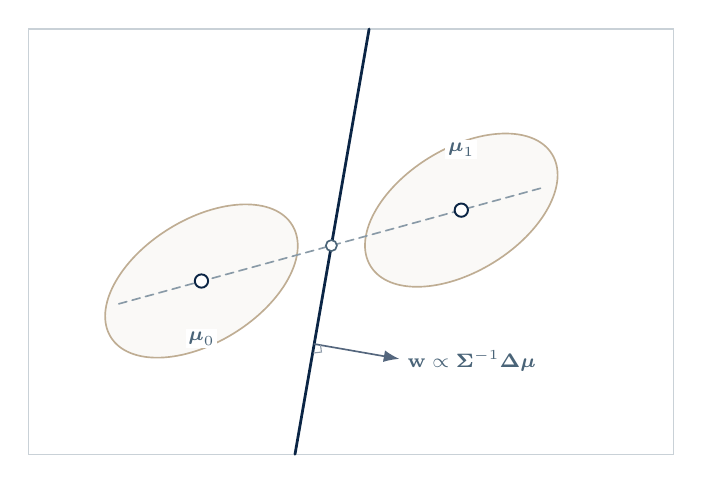
\begin{tikzpicture}[x=1cm,y=1cm,>=Latex,line cap=round]
  \draw[frame] (0,0) rectangle (8.2,5.4);
  % 两个同形椭圆（共享协方差）
  \draw[gold!55,fill=gold!4,line width=0.6pt]
    (2.20,2.20) ellipse [x radius=1.354, y radius=0.781, rotate=31.7];
  \draw[gold!55,fill=gold!4,line width=0.6pt]
    (5.50,3.10) ellipse [x radius=1.354, y radius=0.781, rotate=31.7];
  % 中心连线
  \draw[steel!65,line width=0.6pt,densely dashed] (1.15,1.91) -- (6.55,3.39);
  % 边界
  \draw[navy,line width=1.0pt] (3.388,0) -- (4.329,5.4);
  % 中心
  \fill[white] (2.20,2.20) circle (2.4pt); \draw[navy,line width=0.7pt] (2.20,2.20) circle (2.4pt);
  \fill[white] (5.50,3.10) circle (2.4pt); \draw[navy,line width=0.7pt] (5.50,3.10) circle (2.4pt);
  \node[lab,anchor=north,fill=white,inner sep=1pt] at (2.20,1.60) {$\bmu_0$};
  \node[lab,anchor=south,fill=white,inner sep=1pt] at (5.50,3.74) {$\bmu_1$};
  % 中点（只在图注里说明，不压在线上）
  \fill[white] (3.85,2.65) circle (2.0pt); \draw[steel,line width=0.6pt] (3.85,2.65) circle (2.0pt);
  % w 箭头
  \draw[->,navy!70,line width=0.6pt] (3.632,1.40) -- (4.716,1.211);
  \node[lab,anchor=west] at (4.74,1.19) {$\bw\propto\bSigma^{-1}\bDelta\bmu$};
  % 直角标记：边界与 w
  \draw[navy!45,line width=0.4pt] (3.712,1.386) -- (3.724,1.298) -- (3.626,1.286);
\end{tikzpicture}
\caption{共享协方差下的判别边界。两个椭圆由同一份 $\bSigma$ 生成，只差一个平移——「共享」二字就是这个意思。实线是等先验时的边界：过中点、垂直于 $\bw=\bSigma^{-1}\bDelta\bmu$。注意它\emph{不}垂直于中心连线（虚线）：$\bSigma^{-1}$ 把敏感方向拧向了方差更小的那一侧。}
\label{fig:boundary}
\end{figure}

\begin{keybox}[一句话记住这条边界]
边界是「\textbf{白化空间里的中垂线}」：先用 $\bSigma^{-1/2}$ 把数据压成各向同性，两类中心在那边变成 $\bSigma^{-1/2}\bmu_0$ 与 $\bSigma^{-1/2}\bmu_1$，边界就是它们的中点垂线；再变换回来，中垂线仍然是超平面，只是法向从 $\bDelta\bmu$ 变成了 $\bSigma^{-1}\bDelta\bmu$。

这也解释了为什么「共享 $\bSigma$」是边界线性的\textbf{全部原因}：留一个 $\bSigma$ 给所有类，$-\frac12\log\abs{\bSigma}$ 才能被丢掉，二次项 $\bx\tp\bSigma^{-1}\bx$ 才能在相减时抵消。§7.1 会看到，这两个抵消一个都不能少。
\end{keybox}

\paragraph{回到第二讲：同一个方向。}把 \eqref{eq:scale} 的 $\bSigma=\bS_w/N$ 代进 \eqref{eq:wb}：
\[
  \bw=\bSigma^{-1}\Delta\bmu=N\,\bS_w^{-1}\Delta\bmu\ \propto\ \bS_w^{-1}\Delta\bmu ,
\]
正是第二讲 §3 由 Fisher 准则求出的那个方向。\textbf{两个出发点，同一个法向}：LDA 问「哪个方向使类间散度与类内散度之比最大」，GDA 问「哪一类的密度更高」，两条路在「各类同形」这一点上会合。

因子 $N$ 只改变 $\bw$ 的长度，而 $b$ 会同步乘上 $N$，边界的位置分毫不动——这正是 §4.4 那条尺度警告的另一面：比例因子可以随便丢，前提是\textbf{两边一起丢}。

\subsection{先验的平移量}

\eqref{eq:wb} 里 $\log(\phi_1/\phi_0)$ 是一\emph{纯数}，加在 $\bw\tp\bx$ 这个带量纲的量上。它的几何含义是\textbf{沿法向平移}：

\begin{prop}[先验的平移量]
等先验时（$\phi_1=\phi_0$），边界过两中心的中点。
若 $\phi_1\ne\phi_0$，边界沿 $\bw$ 方向从中点平移
\begin{equation}
  d=\frac{1}{\norm{\bw}}\log\frac{\phi_1}{\phi_0},
  \label{eq:shift}
\end{equation}
方向由 $\phi_1>\phi_0$ 决定：先验大的那一类，其判定区域扩大。
\end{prop}

\begin{proof}
把 \eqref{eq:wb} 写成 $\bw\tp\bigl(\bx-\bx_0\bigr)=0$ 的形式，其中 $\bx_0=\frac{\bmu_1+\bmu_0}{2}-\frac{\log(\phi_1/\phi_0)}{\norm{\bw}^2}\bw$。第二项就是沿 $-\bw$ 方向的平移，长度即 \eqref{eq:shift}。
\end{proof}

两件事要分清：\textbf{先验只平移边界，不改变法向}。法向由 $\bSigma^{-1}\bDelta\bmu$ 决定，与 $\phi$ 无关；$\phi$ 只决定边界落在哪里。这与下一讲（逻辑回归）的情形一致——那里截距吸收了先验，而斜率的含义不变。

% ============================================================
%  第 7 节
% ============================================================

\section{协方差约束的两个维度}

到这里，$\bSigma$ 一直按「所有类共享同一个、且不设任何结构」来处理。这一节问：如果松开，会得到什么？如果收紧，又会怎样？

教材通常把 QDA、GDA、朴素贝叶斯排成「从强到弱」的三级阶梯，暗示参数逐级减少。\hl{这是错的}——约束其实有\emph{两个}独立的维度，四个格子之间只有两条链各自单调，链与链之间不可比。

\subsection{两个约束维度}

第一个维度是\textbf{是否共享}：所有类共用一个 $\bSigma$，还是每类各自一个 $\bSigma_c$。第二个维度是\textbf{是否对角}：允许各维之间相关（满矩阵），还是强制不相关（对角）。

两维独立，于是有四个格子：

\begin{center}
\small
\begin{tabular}{@{}lccl@{}}
\toprule
\rowcolor{navy!7}
\tabhead 协方差结构 & \tabhead 每类的自由参数 & \tabhead 名称 & \tabhead 边界\\
\midrule
共享 $\cdot$ 满 & $\frac{D(D+1)}{2}$ & GDA（本讲） & 超平面\\
各类 $\cdot$ 满 & $K\frac{D(D+1)}{2}$ & QDA & 二次曲面\\
共享 $\cdot$ 对角 & $D$ & 共享对角 & 超平面\\
各类 $\cdot$ 对角 & $KD$ & Gaussian 朴素贝叶斯 & 二次曲面\\
\bottomrule
\end{tabular}
\end{center}

加上先验的 $K-1$ 与均值的 $KD$，四格的总参数为

\begin{center}
\small
\begin{tabular}{@{}lcccc@{}}
\toprule
\rowcolor{navy!7}
\tabhead $(D,K)$ & \tabhead 共享 $\cdot$ 对角 & \tabhead 共享 $\cdot$ 满 & \tabhead 各类 $\cdot$ 对角 & \tabhead 各类 $\cdot$ 满\\
\midrule
$(2,2)$   & $\mathbf{7}$ & $8$   & $9$   & $11$\\
$(10,3)$  & $\mathbf{42}$ & $87$  & $62$  & $197$\\
$(50,5)$  & $\mathbf{304}$ & $1529$ & $504$ & $6629$\\
\bottomrule
\end{tabular}
\end{center}

\begin{keybox}[「对角更省参数」只在同一条链内成立]
沿「共享 $\to$ 各类」看，参数乘 $K$；沿「满 $\to$ 对角」看，参数从 $\frac{D(D+1)}{2}$ 降到 $D$。两条链各自单调，但\textbf{链与链之间没有序}。

看 $(D,K)=(2,2)$ 那一行：「各类 $\cdot$ 对角」要 $9$ 个参数，比「共享 $\cdot$ 满」的 $8$ 个还多一个。原因是每类各估一组方差会乘以 $K$，而共享满矩阵只要一份 $\frac{D(D+1)}{2}$。两者的交叉点在
\[
  KD=\frac{D(D+1)}{2}\quad\Longleftrightarrow\quad K=\frac{D+1}{2}.
\]
$K$ 小于这个值时对角吃亏，大于时对角占便宜。$(10,3)$ 与 $(50,5)$ 两行都满足 $K<\frac{D+1}{2}$，所以对角更省；$(2,2)$ 不满足，于是反过来了。
\end{keybox}

这张表还解释了一件实践中的事：为什么「共享 $\cdot$ 对角」这一格虽然最省参数，却常常不是首选。它同时假设了「各类同形」与「各维独立」，两条都强；省下的参数未必抵得上两次判断错误的风险。省参数与少犯错是两件事。

\subsection{各类独立的满协方差}

去掉「共享」，允许 $\bSigma_c$ 各不相同。此时 $-\frac12\log\abs{\bSigma_c}$ 与 $\bx\tp\bSigma_c^{-1}\bx$ 都\emph{不能}再丢掉，判别函数是

\begin{equation}
  \delta_c^{\mathrm{QDA}}(\bx)
  =-\tfrac12\log\abs{\bSigma_c}
  -\tfrac12(\bx-\bmu_c)\tp\bSigma_c^{-1}(\bx-\bmu_c)+\log\phi_c .
  \label{eq:qda}
\end{equation}

第二讲 §4.4 只点到「松开共享就得到 QDA」，没有展开参数估计——那里 $\bSigma_c$ 的 MLE 就是把 \eqref{eq:mleSigma} 按类各算一遍。这里只看它的结构：与 \eqref{eq:delta} 相比多了两样东西，\textbf{一个依赖 $c$ 的行列式项}（体积惩罚）与\textbf{一个依赖 $c$ 的二次型}。两项都随 $c$ 变，所以相减时消不掉，边界成了两个二次型相等——一般是一条二次曲线。

一个常被忽略的后果：QDA 的判别区域\textbf{可以有界}。若某类的 $\abs{\bSigma_c}$ 明显大于其他类，它的「体积惩罚」就更重，远离所有数据中心的地方会倾向判给协方差小的那一类。这意味着 QDA 的外推行为依赖方向，而不像超平面那样稳定。样本外的预测要格外小心。

\subsection{共享的满协方差}

就是前面五节做的事，在四格里位于「共享 $\cdot$ 满」。它在表里不是「中间一档」，而是两条链的一个交点：与 QDA 共享「满」，与对角格共享「共享」。

它的两条性质都来自「共享」这一个字，值得并排看：

\begin{itemize}
  \item $-\frac12\log\abs{\bSigma}$ 与 $c$ 无关 $\Rightarrow$ 可以丢掉 $\Rightarrow$ 不产生体积惩罚；
  \item $\bx\tp\bSigma^{-1}\bx$ 与 $c$ 无关 $\Rightarrow$ 相减时抵消 $\Rightarrow$ 边界是超平面。
\end{itemize}

两条都是「同一个矩阵被所有类使用」的直接推论。少了任一条，边界就不再是直线。

\subsection{各格的对角版本}

把满矩阵换成对角阵 $\bSigma_c=\diag(\sigma_{c1}^2,\dots,\sigma_{cD}^2)$，二次型立刻裂成逐维之和：

\begin{equation}
  \delta_c^{\mathrm{NB}}(\bx)
  =-\frac12\sum_{j=1}^{D}\log\sigma_{cj}^2
  -\frac12\sum_{j=1}^{D}\frac{\bigl(x^{(j)}-\mu_c^{(j)}\bigr)^2}{\sigma_{cj}^2}
  +\log\phi_c .
  \label{eq:gnb}
\end{equation}

这正对应「给定类别时，各维条件独立」这一假设——联合密度是边缘密度的乘积，取对数就变成求和。所谓「朴素」，朴素在这里。

边界形状有一个可以从图上一眼认出的特征：\textbf{二次项只含 $(x^{(j)})^2$，没有 $x^{(j)}x^{(k)}$ 交叉项}。因此二次曲面的主轴\emph{平行于坐标轴}。QDA 的主轴一般不平行。这是分辨两者的最快办法。

若再进一步，连方差也共享（$\sigma_{cj}^2=\sigma_j^2$），则每类的二次项只差一个平移，相减时消去：

\begin{equation}
  \delta_c^{\mathrm{sh}}(\bx)=\sum_{j=1}^{D}\frac{x^{(j)}\mu_c^{(j)}}{\sigma_j^2}
  -\frac12\sum_{j=1}^{D}\frac{\bigl(\mu_c^{(j)}\bigr)^2}{\sigma_j^2}+\log\phi_c ,
  \label{eq:shareddiag}
\end{equation}
又是线性的。这就是四格表里最省参数的那一格。

\begin{add}[对角假设的两个代价]
\begin{enumerate}[label=\textcolor{steel}{\bfseries(\arabic*)},leftmargin=2.2em]
  \item \textbf{丢掉相关结构}。若两维高度相关，对角模型会把同一份信息数两遍，等价于给这一对特征加了权。特征重复时，这一点尤其明显。
  \item \textbf{坐标依赖}。对角是相对于当前坐标系说的：把数据旋转 45°，对角假设的含义就完全变了。这意味着「朴素贝叶斯效果好」有时只是坐标系选得巧，而不是假设真的成立。
\end{enumerate}
\end{add}

% ============================================================
%  第 8 节
% ============================================================

\section{失效与诊断}

前面所有的推导都建立在三条假设上：每一类是高斯、协方差共享、$\bS$ 可逆。这一节逐条问：假设不成立时，错在哪、怎么看出来、怎么补救。

\subsection{高斯假设的偏离}

高斯假设有三处容易被违反，症状各不相同：

\begin{center}
\small
\begin{tabular}{@{}p{2.9cm}p{4.4cm}p{5.2cm}@{}}
\toprule
\rowcolor{navy!7}
\tabhead 偏离形态 & \tabhead 典型来源 & \tabhead 后果\\
\midrule
重尾 & 含离群点的连续特征 & 均值与协方差都被拉偏，边界整体位移\\
多峰 & 类内还有未观测的子群 & 一个高斯的单峰会「架在两峰之间」，边界穿过数据密度低谷\\
形状不同 & 各类的协方差确实不同 & 共享 $\bSigma$ 被最松散的那一类拽走，法向朝它偏\\
\bottomrule
\end{tabular}
\end{center}

诊断的入手点都一样：\textbf{逐类看边际分布}。对每一维、每个类画直方图或 Q-Q 图；偏度大、尾部远超直线，就说明高斯假设在那一维上不成立。

第二条要单独检查：\textbf{各类的协方差是否相近}。比较 $\tr(\bS_c)$ 与 $\abs{\bS_c}$ 的量级，差异明显时，共享假设就值得怀疑——此时应当考虑 §7.2 的 QDA（各类独立），或者先对每类做白化再合并。这一条的正式检验叫 Box's $M$，但它对非正态极其敏感，实践中靠量级比较已经够用。

\begin{warn}[共享协方差的失败不显眼]
重尾和多峰一眼能看出来，共享协方差的失败却常常看不出来：训练集上准确率照旧很高，因为边界只要落在两类之间的空隙里就行。真正暴露问题的是\emph{新样本}，尤其是落在两类中间的样本——那里的判定方向由 $\bSigma$ 决定，而 $\bSigma$ 已经被最大的一类主导了。

一个便宜的检查：把 $\bS_c$ 逐个算出来，看它们的主特征向量方向是否一致。方向差异大，说明共享假设在几何上就不成立。
\end{warn}

\subsection{协方差奇异}

判据要按格分开写，混用是最常见的错误。

\begin{center}
\small
\begin{tabular}{@{}lll@{}}
\toprule
\rowcolor{navy!7}
\tabhead 情形 & \tabhead 秩的上界 & \tabhead 满秩条件\\
\midrule
共享 $\hat\bSigma$（GDA） & $N-K$ & $N-K\ge D$\\
每类 $\bS_c$（QDA） & $N_c-1$ & $N_c\ge D+1$\\
对角（朴素贝叶斯） & — & $N_c\ge2$，且该维方差非零\\
\bottomrule
\end{tabular}
\end{center}

第一行常被写错。看到「每类只有两个点」就断言协方差奇异，是把 QDA 的门槛安到了 GDA 头上：共享估计把各类的离差加在一起，
\[
  \rank\Bigl(\sum_c N_c\bS_c\Bigr)\le\sum_c(N_c-1)=N-K,
\]
所以只要\textbf{总样本量够了就满秩，与单个类有多大无关}。$D=4$、$N_1=2$、$N_2=100$ 时第一类只有两个点，$\hat\bSigma$ 照样可逆。

C 形判据（$N-K<D$）出现时，补救按代价从小到大排：

\begin{enumerate}[label=\textcolor{navy}{\bfseries\arabic*.},leftmargin=2.2em]
  \item \textbf{对角加载} $\bSigma+\lambda\bI$：一行代码，立刻可逆，代价是引入偏差。$\lambda$ 从 $10^{-6}$ 起步，按条件数涨到 $10^{-2}$ 量级（§5.3）。
  \item \textbf{向共享收缩}：若只是某一类的 $\bS_c$ 奇异，把它拉向 $\bSigma$ 即可（§5.3 的 $\alpha$）。
  \item \textbf{先降维再判别}：用主成分把 $D$ 压到 $N-K$ 以下。这一条要谨慎——降维的方向由无监督的方差决定，未必与判别有关。
\end{enumerate}

\begin{add}[两个信号的区分]
「$\bS$ 奇异」与「$\bS$ 病态」是两件事，处理方式不同。

奇异的信号很明确：Cholesky 分解报错，或某个特征值数值上恰好为零。病态则隐蔽得多：矩阵可逆，但条件数 $10^{10}$，求逆之后误差被放大到不可用。后者的症状是系数剧烈摆动、换一批样本边界就大变。

判断办法是看特征值谱，而不是看是否报错。$\lambda_{\max}/\lambda_{\min}>10^{6}$ 时就该考虑正则化了。
\end{add}

\subsection{与逻辑回归的取舍}

共享协方差的高斯假设，等价于「对数几率是线性的」。第四讲会把这条结论单独取出来，丢掉其余全部假设，只留下它。逐项对照在第二讲 \S4.5 与第四讲 \S7.2 的两张表里，本节不重复列第三张。

这里只补一件那两张表没有量化的东西：\textbf{参数的阶}。

GDA 要 $(K-1)+KD+\frac{D(D+1)}{2}$ 个参数，逻辑回归要 $(K-1)(D+1)$ 个。取 $D=50$、$K=2$，前者是 $1+100+1275=1376$，后者是 $1\times 51=51$。差别几乎全部来自 $\frac{D(D+1)}{2}$ 这一项——它随维数\textbf{平方}增长，而其余部分都是线性的。

这个阶数差解释了经验规律的边界。假设成立时，那 $D^2$ 个参数是划算的：每一个都能被类内离差估准，而且估完之后边界是算出来的，不必搜索。假设不成立时，同样的 $D^2$ 个参数就变成了 $D^2$ 个偏差来源——它们没有一个在描述真实形状，却都进了 $\bSigma^{-1}$。

换句话说，\textbf{生成式的赌注是随维数平方增长的}。维数越高，赌对赚得越多，赌错输得越惨。这也是为什么在高维稀疏的场合（文本是典型），人们宁可退回朴素贝叶斯的对角假设：不是因为它更对，而是因为它把 $D^2$ 降成了 $D$。

\begin{keybox}[什么时候不该用 GDA]
三条同时成立时才用：
\begin{enumerate}[label=\textcolor{navy}{\bfseries(\arabic*)},leftmargin=2.2em]
  \item 特征大致连续、逐类的边际分布接近单峰对称；
  \item 各类的协方差形状相近（否则至少要走 QDA）；
  \item 样本量足以支撑 $D(D+1)/2$ 个协方差参数，即 $N-K\gg D$。
\end{enumerate}

任一条明显不成立，先考虑下一讲的判别式路线，或者回到 §5 加正则。\textbf{不要因为「它有闭式解」就选它}——闭式解的代价是把判断押在那三条假设上。
\end{keybox}

% ============================================================
%  第 9 节
% ============================================================

\section{小结}

\subsection{五个要点}

\begin{enumerate}[label=\textcolor{navy}{\bfseries\arabic*.},leftmargin=2.3em,itemsep=0.55em]
  \item \textbf{生成式分类器要估的是联合分布，参数的大头在协方差。}$(K-1)+KD+K\frac{D(D+1)}{2}$ 里，第三项随 $D^2$ 涨，是全部约束手段的战场。
  \item \textbf{三组参数天然可分离。}对数似然按类别分组后，$\phi$ 只进第一项，$\bmu$ 与 $\bSigma$ 只进第二项，所以能逐个闭式求解，不必做联合优化。
  \item \textbf{均值的估计与协方差无关，靠的是一条恒等式。}剖面似然恒等式里交叉项\emph{恒等于零}，不是被一阶条件消掉的——这个区别决定了「先估 $\bmu$ 再估 $\bSigma$」是否合法。
  \item \textbf{协方差的 MLE 是加权平均，推导的关键是迹技巧。}$\sum_i$ 个二次型被压成 $\tr(\bS\bSigma^{-1})$，之后求导只是套公式。注意「右乘 $\bSigma^2$」那种写法过程错、结论对，错得还很系统。
  \item \textbf{边界线性来自「共享」二字。}共享使 $-\frac12\log\abs{\bSigma}$ 可丢、使 $\bx\tp\bSigma^{-1}\bx$ 相消；法向是 $\bSigma^{-1}\bDelta\bmu$ 而非 $\bDelta\bmu$，先验只平移、不改法向。
\end{enumerate}

\subsection{知识结构}

\begin{figure}[htbp]
\centering
\begingroup
\providecommand{\ttl}{\bfseries\sffamily\color{navy}}
\providecommand{\fml}{\footnotesize\color{navy!88}}
\begin{tikzpicture}[
  box/.style={draw=navy!55,fill=navy!3,minimum width=2.55cm,minimum height=1.95cm,
    align=center,inner sep=2pt,sharp corners,line width=0.5pt},
  ar/.style={->,navy!60,line width=0.6pt},
]
\node[box] (b1) at (1.45,0) {{\ttl 假设}\\[2pt]{\fml $\bx\mid y=c\sim\Ncal(\bmu_c,\bSigma)$}\\[0pt]{\fml $y\sim\mathrm{Bern}(\phi)$}};
\node[box] (b2) at (4.55,0) {{\ttl 似然}\\[2pt]{\fml 按 $y_i$ 分组}\\[0pt]{\fml 三组可分离}};
\node[box] (b3) at (7.65,0) {{\ttl 估计}\\[2pt]{\fml $\hat\phi_c=N_c/N$}\\[0pt]{\fml $\hat\bmu_c=\bar\bx_c$}};
\node[box] (b4) at (10.75,0) {{\ttl 协方差}\\[2pt]{\fml 迹技巧}\\[0pt]{\fml $\hat\bSigma=\frac1N\sum_c N_c\bS_c$}};
\node[box] (b5) at (13.85,0) {{\ttl 判定}\\[2pt]{\fml 三项得分}\\[0pt]{\fml $w=\bSigma^{-1}\Delta\bmu$}};
\draw[ar] (b1) -- (b2);
\draw[ar] (b2) -- (b3);
\draw[ar] (b3) -- (b4);
\draw[ar] (b4) -- (b5);
% 下方：四格
\node[draw=navy!25,fill=white,align=center,font=\footnotesize,inner sep=5pt]
  at (7.65,-2.55)
  {共享 / 各自 $\ \times\ $ 满 / 对角 $=$ 四格 \quad $\cdot$ \quad 只有「共享 $\cdot$ 满」给出超平面};
\draw[<->,navy!45,line width=0.55pt,densely dashed] (b1.south) to[bend right=18] (b4.south);
\end{tikzpicture}
\endgroup
\caption{五个节点就是这一讲的五个动作，从左到右单向走完。中间那条虚线是唯一一次回头：对 $\bSigma$ 的假设动一下，前面的分组结构与后面的边界形状会同时变，所以「松假设」不能只改一处。}
\label{fig:map}
\end{figure}

\subsection{后续内容}

这一讲停在「共享协方差的满矩阵」上。往下有四条路：

\begin{itemize}
  \item \textbf{丢掉高斯假设}。下一讲只保留「对数几率线性」这一条结论，其余全部丢弃。有趣的是，那条结论恰是共享协方差高斯的\emph{推论}——所以凡是 GDA 站得住的地方，逻辑回归都成立，反过来则不然。
  \item \textbf{换成条件独立假设}。若特征是离散的、维数很高（文本是典型），对角假设仍然估不动，于是进一步假设给定类别时各维独立——那就是朴素贝叶斯，与 §7.4 的 Gaussian NB 是同一件事在不同数据类型上的形态。
  \item \textbf{把约束连续化}。§5.3 的 $\alpha$ 只在「共享」与「各自」之间插值。现代的收缩估计（Ledoit–Wolf 一类）进一步把收缩强度做成数据驱动的，不再靠交叉验证挑。
  \item \textbf{非线性边界}。QDA 只是二次曲面。再往前是核方法与神经网络：先做一个非线性映射 $\varphi$，在那边画超平面，回到原空间就成了曲面。骨架一点没变，仍是 $\bw\tp\varphi(\bx)$。
\end{itemize}

% ============================================================
%  习题
% ============================================================

\clearpage
\section*{习题}
\addcontentsline{toc}{section}{习题}
\markboth{习题}{}
\setlength{\parskip}{0.62em}

\subsection*{A 组 · 基础}

\noindent\textbf{A1.} 用拉格朗日乘子解 \eqref{eq:phiobj}，并说明为什么不能直接令 $N_c/\phi_c=0$。若约束改成 $\sum_c\phi_c^2=1$，解会变成什么？

\noindent\textbf{A2.} 写出 $K$ 类 GDA 的参数个数，并算出 $(D,K)=(6,4)$ 的值；再算出同配置下 QDA 与 Gaussian 朴素贝叶斯的参数个数，排出大小顺序。

\noindent\textbf{A3.} 取 $\bA=\begin{pmatrix}2&1\\1&3\end{pmatrix}$，$\bB=\begin{pmatrix}1&0\\0&2\end{pmatrix}$。验证 \eqref{eq:trace1} 的迹技巧：先算 $\ba\tp\bA^{-1}\ba$，再算 $\tr(\bA^{-1}\ba\ba\tp)$，确认两者相等。再验证 \eqref{eq:dinv} 给出的梯度与逐元素求导（非对角元乘 $2$）一致。

\noindent\textbf{A4.} 从 \eqref{eq:delta} 出发，证明它等价于「按马氏距离找最近的类中心，并按 $-\log\phi_c$ 加权」。提示：把 $\delta_c$ 写成 $-\frac12\norm{\bx-\bmu_c}^2_{\bSigma}+\log\phi_c$ 加一个与 $c$ 无关的项。

\noindent\textbf{A5.} 设 $\phi_1=0.8$、$\phi_0=0.2$，$\norm{\bw}=4$。边界沿法向平移多少？朝哪一侧？若两类的先验反转为 $0.2/0.8$，边界移动的距离是多少？

\subsection*{B 组 · 提高}

\noindent\textbf{B1.} 证明剖面似然恒等式 \eqref{eq:profile}，并说明为什么它使「先估 $\bmu$ 再估 $\bSigma$」不构成循环论证。若交叉项不恒为零，推导会在哪一步卡住？

\noindent\textbf{B2.} 证明定理 4.1 的驻点是\emph{唯一}全局极大点。提示：先证 $F(\bSigma)=\frac N2\log\abs{\bSigma}+\frac N2\tr(\bS\bSigma^{-1})$ 在 $\bSigma\succ0$ 上是凸的（可用 $\bSigma$ 的特征值把 $F$ 写成逐特征值的函数），再用一阶条件。

\noindent\textbf{B3.} 说明为什么「右乘 $\bSigma^2$」那种错误写法\emph{总能}给出正确答案。设目标形如 $-\frac a2\log\abs{\bSigma}-\frac b2\tr(\bM\bSigma^{-1})$，分别写出错误梯度与正确梯度对应的驻点方程，证明两者等价。再举一个「错误不再被抵消」的目标函数。

\noindent\textbf{B4.} 证明 §7.4 的断言：对角协方差下，二次曲面的主轴平行于坐标轴。提示：写出边界的二次型，检查 $x^{(j)}x^{(k)}$（$j\ne k$）的系数。

\noindent\textbf{B5.} 证明：Gaussian 朴素贝叶斯比 GDA 省参数的充要条件是 $K<\frac{D+1}{2}$。再说明这个不等式为什么只比较了「各类 $\cdot$ 对角」与「共享 $\cdot$ 满」两格，而不能推出四格的完整排序。

\subsection*{C 组 · 动手}

\noindent\textbf{C1.} 不用现成库，实现二类 GDA：用 Cholesky 分解算 $\log\det\bSigma$ 与 $\bSigma^{-1}\bDelta\bmu$，用 logsumexp 算后验，并在某个标准数据集上与 \texttt{sklearn} 的 \texttt{LinearDiscriminantAnalysis} 对齐到 $10^{-8}$（注意它默认对协方差做缩放，先确认口径）。

\noindent\textbf{C2.} 造一份 $D=40$、$N=50$ 的两类数据，令 $N-K<D$。报告 $\bS$ 的最小特征值与条件数；再画出 $\lambda$ 从 $10^{-8}$ 到 $10^{1}$ 时条件数与测试准确率的两条曲线，找出「可逆但不可用」的区间。

\noindent\textbf{C3.} 在同一份二维数据上分别用 QDA、GDA、Gaussian 朴素贝叶斯拟合，把三条边界画在一张图上，标出各自的主轴方向。构造一份数据使三者的训练错分数相同而边界明显不同。

\noindent\textbf{C4.} 检查共享协方差假设：对每一类算 $\bS_c$，报告主特征向量之间的夹角与 $\tr(\bS_c)$ 的比值。再人为把某一类的散布放大三倍，观察 GDA 的边界朝哪一侧偏，并解释原因。

\subsection*{提示}

\begin{itemize}[itemsep=0.2em]
  \item \textbf{A1}：$\lambda=N$；改成平方约束后，解变成 $\phi_c\propto N_c^{1/2}$，注意归一化。
  \item \textbf{A2}：$(6,4)$ 时 GDA 为 $3+24+21=48$，QDA 为 $3+24+84=111$，NB 为 $3+24+24=51$；顺序是 GDA $<$ NB $<$ QDA。
  \item \textbf{A3}：$\bA^{-1}=\frac15\begin{pmatrix}3&-1\\-1&2\end{pmatrix}$，做完两次计算会发现只差一个转置位置。
  \item \textbf{A4}：$\norm{\bx-\bmu_c}^2_{\bSigma}=\bx\tp\bSigma^{-1}\bx-2\bx\tp\bSigma^{-1}\bmu_c+\bmu_c\tp\bSigma^{-1}\bmu_c$，第一项与 $c$ 无关。
  \item \textbf{A5}：$d=\frac14\log4\approx0.347$，朝使类 $1$ 区域扩大的一侧；反转后移动同样距离，方向相反。
  \item \textbf{B2}：令 $\bSigma=\bU\diag(\lambda_j)\bU\tp$，则 $F=\frac N2\sum_j\bigl(\log\lambda_j+s_j/\lambda_j\bigr)$，其中 $s_j$ 是 $\bS$ 在同一组特征向量下的对角元——先把 $\bS$ 与 $\bSigma$ 同时对角化，再用 $x\mapsto\log x+s/x$ 的凸性。
  \item \textbf{B3}：错式给 $a\bSigma^{-1}=b\bM\bSigma^{-2}$，右乘 $\bSigma^2$ 得 $a\bSigma=b\bM$；对式左乘右乘各一次也得 $a\bSigma=b\bM$。反例：目标含 $\tr(\bM\bSigma^{-1}\bN\bSigma^{-1})$ 时两者不再等价。
  \item \textbf{B4}：边界是 $\sum_j\bigl[\frac{1}{\sigma_{1j}^2}-\frac{1}{\sigma_{0j}^2}\bigr](x^{(j)})^2+\cdots=0$，交叉项系数为零。
  \item \textbf{B5}：比较 $KD$ 与 $\frac{D(D+1)}{2}$；两格分别属于不同的链，所以这个不等式不能推广成四格的排序。
  \item \textbf{C2}：$\lambda$ 太小时条件数仍在 $10^{10}$ 以上，准确率不升反降；找曲线拐点。
  \item \textbf{C4}：把某一类的 $\bS_c$ 放大后，共享 $\bS$ 被它主导，边界法向朝该类的主轴方向偏。
\end{itemize}

% ============================================================
%  附录
% ============================================================

\appendix
\renewcommand{\thesection}{\Alph{section}}

\section{公式速查}

\subsection*{A.1　多元高斯}

\begin{align}
  p(\bx;\bmu,\bSigma)&=\frac{1}{(2\pi)^{D/2}\abs{\bSigma}^{1/2}}
    \exp\Bigl[-\tfrac12(\bx-\bmu)\tp\bSigma^{-1}(\bx-\bmu)\Bigr],\\
  \log p(\bx;\bmu,\bSigma)&=-\tfrac D2\log(2\pi)-\tfrac12\log\abs{\bSigma}
    -\tfrac12(\bx-\bmu)\tp\bSigma^{-1}(\bx-\bmu).
\end{align}

\subsection*{A.2　本讲用到的三条矩阵求导}

\begin{align}
  \frac{\partial}{\partial\bA}\log\abs{\bA}&=\bigl(\bA^{-1}\bigr)\tp
    \quad(\bA\ \text{对称时}=\bA^{-1}),\\
  \frac{\partial}{\partial\bA}\tr(\bA\bB)&=\bB\tp,\\
  \frac{\partial}{\partial\bA}\tr(\bB\bA^{-1})&=-\bA^{-1}\bB\bA^{-1}
    \quad(\bA,\bB\ \text{对称}).
\end{align}

\subsection*{A.3　估计量}

\begin{align}
  \hat\phi_c&=\frac{N_c}{N},&
  \hat\bmu_c&=\bar\bx_c=\frac1{N_c}\sum_{i:y_i=c}\bx_i,\\
  \hat\bSigma&=\frac1N\sum_c N_c\bS_c=\frac1N\bS_w,&
  \bS_c&=\frac1{N_c}\sum_{i:y_i=c}(\bx_i-\bar\bx_c)(\bx_i-\bar\bx_c)\tp .
\end{align}

\subsection*{A.4　判别与边界}

\begin{align}
  \delta_c(\bx)&=\bx\tp\bSigma^{-1}\bmu_c-\tfrac12\bmu_c\tp\bSigma^{-1}\bmu_c+\log\phi_c,\\
  \bw&=\bSigma^{-1}(\bmu_1-\bmu_0),\\
  b&=-\tfrac12(\bmu_1+\bmu_0)\tp\bSigma^{-1}(\bmu_1-\bmu_0)+\log\frac{\phi_1}{\phi_0},\\
  d_{\text{平移}}&=\frac{1}{\norm{\bw}}\log\frac{\phi_1}{\phi_0}.
\end{align}

\subsection*{A.5　四格的参数量}

\begin{center}
\small
\begin{tabular}{@{}lll@{}}
\toprule
\rowcolor{navy!7}
\tabhead 结构 & \tabhead 协方差个数 & \tabhead 总参数\\
\midrule
共享 $\cdot$ 满 & $\frac{D(D+1)}{2}$ & $(K-1)+KD+\frac{D(D+1)}{2}$\\
共享 $\cdot$ 对角 & $D$ & $(K-1)+KD+D$\\
各类 $\cdot$ 满 & $K\frac{D(D+1)}{2}$ & $(K-1)+KD+K\frac{D(D+1)}{2}$\\
各类 $\cdot$ 对角 & $KD$ & $(K-1)+KD+KD$\\
\bottomrule
\end{tabular}
\end{center}

\section{延伸阅读}

\begin{itemize}
  \item \textbf{判别分析的经典处理}：Hastie, Tibshirani \& Friedman, \emph{The Elements of Statistical Learning}, 第 4.3 节。QDA、RDA 与收缩的来龙去脉在那里最清楚。
  \item \textbf{生成式与判别式的对照}：Ng \& Jordan (2001), \emph{On Discriminative vs.\ Generative Classifiers}。这篇短文把「假设对时生成式更省样本」从口号变成了渐近分析。
  \item \textbf{贝叶斯视角的完整推导}：Bishop, \emph{Pattern Recognition and Machine Learning}, 第 4.2 节（概率生成模型）与第 2.3 节（高斯分布）。逆 Wishart 与 NIW 的后验形式都在那里。
  \item \textbf{朴素贝叶斯的现代讨论}：Zhang (2004), \emph{The Optimality of Naive Bayes}。它解释了为什么「假设明显不成立时朴素贝叶斯仍然好用」。
  \item \textbf{实现参照}：\texttt{sklearn.discriminant\_analysis} 的文档列出了 \texttt{reg\_param} 与收缩的用法，§5.3 的两种做法在里面都能找到对应参数。
\end{itemize}

\end{document}
